%%%%%%%%%%%%%%%%%%%%%%%%%%%%%%%%%%%%%%%%
% datoteka diploma-vzorec.tex
%
% vzorčna datoteka za pisanje diplomskega dela v formatu LaTeX
% na UL Fakulteti za računalništvo in informatiko
%
% vkup spravil Gašper Fijavž, december 2010
% 
%
%
% verzija 12. februar 2014 (besedilo teme, seznam kratic, popravki Gašper Fijavž)
% verzija 10. marec 2014 (redakcijski popravki Zoran Bosnić)
% verzija 11. marec 2014 (redakcijski popravki Gašper Fijavž)
% verzija 15. april 2014 (pdf/a 1b compliance, not really - just claiming, Damjan Cvetan, Gašper Fijavž)
% verzija 23. april 2014 (privzeto cc licenca)
% verzija 16. september 2014 (odmiki strain od roba)
% verzija 28. oktober 2014 (odstranil vpisno številko)
% verija 5. februar 2015 (Literatura v kazalu, online literatura)
% verzija 25. september 2015 (angl. naslov v izjavi o avtorstvu)
% verzija 26. februar 2016 (UL izjava o avtorstvu)
% verzija 16. april 2016 (odstranjena izjava o avtorstvu)
% verzija 5. junij 2016 (Franc Solina dodal vrstice, ki jih je označil s svojim imenom)

% \UseRawInputEncoding
\documentclass[a4paper, 12pt]{book}
%\documentclass[a4paper, 12pt, draft]{book}  Nalogo preverite tudi z opcijo draft, ki vam bo pokazala, katere vrstice so predolge!


\usepackage[utf8]{inputenc}   % omogoča uporabo slovenskih črk kodiranih v formatu UTF-8
\usepackage[slovene,english]{babel}    % naloži, med drugim, slovenske delilne vzorce

\usepackage[
backend=biber,
maxbibnames=9,
]{biblatex}

% If you want to break on URL numbers
\setcounter{biburlnumpenalty}{9000}
% If you want to break on URL lower case letters
\setcounter{biburllcpenalty}{9000}
% If you want to break on URL UPPER CASE letters
\setcounter{biburlucpenalty}{9000}

\addbibresource{literatura.bib}

\usepackage[pdftex]{graphicx}  % omogoča vlaganje slik različnih formatov
\graphicspath{ {./images/} }

\usepackage{float}          % poskrbi, na primer, za glave strani
\usepackage{csquotes}
\DeclareQuoteAlias{german}{english}
\usepackage{fancyhdr}          % poskrbi, na primer, za glave strani
\usepackage{fancyvrb}          % poskrbi za underlined verbatim
\usepackage{amssymb}           % dodatni simboli
\usepackage{amsmath}           % eqref, npr.
\usepackage{hyperxmp}
%\usepackage[hyphens]{url}  % dodal Solina
%\usepackage{comment}       % dodal Solina
\usepackage[pdftex, colorlinks=true,
  						citecolor=black, filecolor=black, 
  						linkcolor=black, urlcolor=black,
  						pagebackref=false, 
  						pdfproducer={LaTeX}, pdfcreator={LaTeX}, hidelinks]{hyperref}
 
%\usepackage[separate-uncertainty=true,multi-part-units=repeat]{siunitx}

\usepackage{color}       % dodal Solina
\usepackage{soul}       % dodal Solina

%%%%%%%%%%%%%%%%%%%%%%%%%%%%%%%%%%%%%%%%
%	DIPLOMA INFO
%%%%%%%%%%%%%%%%%%%%%%%%%%%%%%%%%%%%%%%%
\newcommand{\ttitle}{Avtomatizacija delavniškega dnevnika}
\newcommand{\ttitleEn}{Workshop report automatization}
\newcommand{\tsubject}{\ttitle}
\newcommand{\tsubjectEn}{\ttitleEn}
\newcommand{\tauthor}{Anej Lekše}
\newcommand{\tkeywords}{mobilni razvoj, glasovni pomočniki, razpoznava glasu, informacijski sistemi}
\newcommand{\tkeywordsEn}{mobile development, voice assistants, voice recognition, information systems}


%%%%%%%%%%%%%%%%%%%%%%%%%%%%%%%%%%%%%%%%
%	HYPERREF SETUP
%%%%%%%%%%%%%%%%%%%%%%%%%%%%%%%%%%%%%%%%
\hypersetup{pdftitle={\ttitle}}
\hypersetup{pdfsubject=\ttitleEn}
\hypersetup{pdfauthor={\tauthor, al1617@student.uni-lj.si}}
\hypersetup{pdfkeywords=\tkeywordsEn}


 


%%%%%%%%%%%%%%%%%%%%%%%%%%%%%%%%%%%%%%%%
% postavitev strani
%%%%%%%%%%%%%%%%%%%%%%%%%%%%%%%%%%%%%%%%  

\addtolength{\marginparwidth}{-20pt} % robovi za tisk
\addtolength{\oddsidemargin}{40pt}
\addtolength{\evensidemargin}{-40pt}

\renewcommand{\baselinestretch}{1.3} % ustrezen razmik med vrsticami
\setlength{\headheight}{15pt}        % potreben prostor na vrhu
\renewcommand{\chaptermark}[1]%
{\markboth{\MakeUppercase{\thechapter.\ #1}}{}} \renewcommand{\sectionmark}[1]%
{\markright{\MakeUppercase{\thesection.\ #1}}} \renewcommand{\headrulewidth}{0.5pt} \renewcommand{\footrulewidth}{0pt}
\fancyhf{}
\fancyhead[LE,RO]{\sl \thepage} 
%\fancyhead[LO]{\sl \rightmark} \fancyhead[RE]{\sl \leftmark}
\fancyhead[RE]{\sc \tauthor}              % dodal Solina
\fancyhead[LO]{\sc Diplomska naloga}     % dodal Solina


\newcommand{\BibTeX}{{\sc Bib}\TeX}

%%%%%%%%%%%%%%%%%%%%%%%%%%%%%%%%%%%%%%%%
% naslovi
%%%%%%%%%%%%%%%%%%%%%%%%%%%%%%%%%%%%%%%%  


\newcommand{\autfont}{\Large}
\newcommand{\titfont}{\LARGE\bf}
\newcommand{\clearemptydoublepage}{\newpage{\pagestyle{empty}\cleardoublepage}}
\setcounter{tocdepth}{1}	      % globina kazala

%%%%%%%%%%%%%%%%%%%%%%%%%%%%%%%%%%%%%%%%
% konstrukti
%%%%%%%%%%%%%%%%%%%%%%%%%%%%%%%%%%%%%%%%  
\newtheorem{izrek}{Izrek}[chapter]
\newtheorem{trditev}{Trditev}[izrek]
\newenvironment{dokaz}{\emph{Dokaz.}\ }{\hspace{\fill}{$\Box$}}

%%%%%%%%%%%%%%%%%%%%%%%%%%%%%%%%%%%%%%%%%%%%%%%%%%%%%%%%%%%%%%%%%%%%%%%%%%%%%%%
%% PDF-A
%%%%%%%%%%%%%%%%%%%%%%%%%%%%%%%%%%%%%%%%%%%%%%%%%%%%%%%%%%%%%%%%%%%%%%%%%%%%%%%


%%%%%%%%%%%%%%%%%%%%%%%%%%%%%%%%%%%%%%%% 
% define medatata
%%%%%%%%%%%%%%%%%%%%%%%%%%%%%%%%%%%%%%%% 
\def\Title{\ttitle}
\def\Author{\tauthor, al1617@student.uni-lj.si}
\def\Subject{\ttitleEn}
\def\Keywords{\tkeywordsEn}

%%%%%%%%%%%%%%%%%%%%%%%%%%%%%%%%%%%%%%%% 
% \convertDate converts D:20080419103507+02'00' to 2008-04-19T10:35:07+02:00
%%%%%%%%%%%%%%%%%%%%%%%%%%%%%%%%%%%%%%%% 
\def\convertDate{%
    \getYear
}

{\catcode`\D=12
 \gdef\getYear D:#1#2#3#4{\edef\xYear{#1#2#3#4}\getMonth}
}
\def\getMonth#1#2{\edef\xMonth{#1#2}\getDay}
\def\getDay#1#2{\edef\xDay{#1#2}\getHour}
\def\getHour#1#2{\edef\xHour{#1#2}\getMin}
\def\getMin#1#2{\edef\xMin{#1#2}\getSec}
\def\getSec#1#2{\edef\xSec{#1#2}\getTZh}
\def\getTZh +#1#2{\edef\xTZh{#1#2}\getTZm}
\def\getTZm '#1#2'{%
    \edef\xTZm{#1#2}%
    \edef\convDate{\xYear-\xMonth-\xDay T\xHour:\xMin:\xSec+\xTZh:\xTZm}%
}

\expandafter\convertDate\pdfcreationdate 

%%%%%%%%%%%%%%%%%%%%%%%%%%%%%%%%%%%%%%%%
% get pdftex version string
%%%%%%%%%%%%%%%%%%%%%%%%%%%%%%%%%%%%%%%% 
\newcount\countA
\countA=\pdftexversion
\advance \countA by -100
\def\pdftexVersionStr{pdfTeX-1.\the\countA.\pdftexrevision}


%%%%%%%%%%%%%%%%%%%%%%%%%%%%%%%%%%%%%%%%
% XMP data
%%%%%%%%%%%%%%%%%%%%%%%%%%%%%%%%%%%%%%%%  
\usepackage{xmpincl}
\includexmp{pdfa-1b}

%%%%%%%%%%%%%%%%%%%%%%%%%%%%%%%%%%%%%%%%
% pdfInfo
%%%%%%%%%%%%%%%%%%%%%%%%%%%%%%%%%%%%%%%%  
\pdfinfo{%
    /Title    (\ttitle)
    /Author   (\tauthor, damjan@cvetan.si)
    /Subject  (\ttitleEn)
    /Keywords (\tkeywordsEn)
    /ModDate  (\pdfcreationdate)
    /Trapped  /False
}


%%%%%%%%%%%%%%%%%%%%%%%%%%%%%%%%%%%%%%%%%%%%%%%%%%%%%%%%%%%%%%%%%%%%%%%%%%%%%%%
%%%%%%%%%%%%%%%%%%%%%%%%%%%%%%%%%%%%%%%%%%%%%%%%%%%%%%%%%%%%%%%%%%%%%%%%%%%%%%%

\begin{document}
\selectlanguage{slovene}
\frontmatter
\setcounter{page}{1} %
\renewcommand{\thepage}{}       % preprecimo težave s številkami strani v kazalu
\newcommand{\sn}[1]{"`#1"'}                    % dodal Solina (slovenski narekovaji)

%%%%%%%%%%%%%%%%%%%%%%%%%%%%%%%%%%%%%%%%
%naslovnica
 \thispagestyle{empty}%
   \begin{center}
    {\large\sc Univerza v Ljubljani\\%
      Fakulteta za računalništvo in informatiko}%
    \vskip 10em%
    {\autfont \tauthor\par}%
    {\titfont \ttitle \par}%
    {\vskip 3em \textsc{DIPLOMSKO DELO\\[5mm]         % dodal Solina za ostale študijske programe
    VISOKOŠOLSKI STROKOVNI ŠTUDIJSKI PROGRAM\\ PRVE STOPNJE\\ RAČUNALNIŠTVO IN INFORMATIKA}\par}%
%    UNIVERZITETNI  ŠTUDIJSKI PROGRAM\\ PRVE STOPNJE\\ RAČUNALNIŠTVO IN INFORMATIKA}\par}%
%    INTERDISCIPLINARNI UNIVERZITETNI\\ ŠTUDIJSKI PROGRAM PRVE STOPNJE\\ RAČUNALNIŠTVO IN MATEMATIKA}\par}%
%    INTERDISCIPLINARNI UNIVERZITETNI\\ ŠTUDIJSKI PROGRAM PRVE STOPNJE\\ UPRAVNA INFORMATIKA}\par}%
%    INTERDISCIPLINARNI UNIVERZITETNI\\ ŠTUDIJSKI PROGRAM PRVE STOPNJE\\ MULTIMEDIJA}\par}%
    \vfill\null%
    {\large \textsc{Mentor}: dr.  Andrej Brodnik\par}%
   %{\large \textsc{Somentor}:  izr.\ prof.\ dr. Martin Krpan \par}%
    {\vskip 2em \large Ljubljana, 2020 \par}%
\end{center}
% prazna stran
%\clearemptydoublepage      % dodal Solina (izjava o licencah itd. se izpiše na hrbtni strani naslovnice)

%%%%%%%%%%%%%%%%%%%%%%%%%%%%%%%%%%%%%%%%
%copyright stran
\thispagestyle{empty}
\vspace*{8cm}

\noindent
{\sc Copyright}. 
Rezultati diplomske naloge so intelektualna lastnina avtorja in Fakultete za računalništvo in informatiko Univerze v Ljubljani.
Za objavo in koriščenje rezultatov diplomske naloge je potrebno pisno privoljenje avtorja, Fakultete za računalništvo in informatiko ter mentorja.

\begin{center}
\mbox{}\vfill
\emph{Besedilo je oblikovano z urejevalnikom besedil \LaTeX.}
\end{center}
% prazna stran
\clearemptydoublepage

%%%%%%%%%%%%%%%%%%%%%%%%%%%%%%%%%%%%%%%%
% stran 3 med uvodnimi listi
\thispagestyle{empty}
\vspace*{4cm}

\noindent
Fakulteta za računalništvo in informatiko izdaja naslednjo nalogo:
\medskip
\begin{tabbing}
\hspace{32mm}\= \hspace{6cm} \= \kill




Tematika naloge:
\end{tabbing}
%Besedilo teme diplomskega dela študent prepiše iz študijskega informacijskega sistema, kamor ga je vnesel mentor. V nekaj stavkih bo opisal, kaj pričakuje od kandidatovega diplomskega dela. Kaj so cilji, kakšne metode uporabiti, morda bo zapisal tudi ključno literaturo.
Preveri, ali so glasovni pomočniki v trenutnem stanju primerni za pomoč pri pisanju delavniških dnevnikov.
Seznani se z obstoječimi rešitvami za sestavljanje delavniških dnevnikov in jih analiziraj.
Po analizi področja se loti izdelave svojega sistema za sestavljanje delavniških dnevnikov, ki vključuje glasovnega pomočnika.
\vspace{15mm}



\vspace{2cm}

% prazna stran
\clearemptydoublepage

% zahvala
\thispagestyle{empty}\mbox{}\vfill\null\it%
\noindent
Zahvaljujem se mentorju dr. Andreju Brodniku za odlično usmerjanje pri delu, očetu in mami za neizmerno podporo, Roku Bermežu in podjetju Hisense Gorenje Europe za slikovno gradivo in pomoč.

Hvala vsem.
\rm\normalfont

% prazna stran
\clearemptydoublepage

%%%%%%%%%%%%%%%%%%%%%%%%%%%%%%%%%%%%%%%%
% posvetilo, če sama zahvala ne zadošča :-)
\thispagestyle{empty}\mbox{}{\vskip0.20\textheight}\mbox{}\hfill\begin{minipage}{0.55\textwidth}%
% Svoji dragi Alenčici.
	Meti. Tii. Hvala.
\normalfont\end{minipage}

% prazna stran
\clearemptydoublepage


%%%%%%%%%%%%%%%%%%%%%%%%%%%%%%%%%%%%%%%%
% kazalo
\pagestyle{empty}
\def\thepage{}% preprecimo tezave s stevilkami strani v kazalu
\tableofcontents{}


% prazna stran
\clearemptydoublepage

%%%%%%%%%%%%%%%%%%%%%%%%%%%%%%%%%%%%%%%%
% seznam kratic

\chapter*{Seznam uporabljenih kratic}  % spremenil Solina, da predolge vrstice ne gredo preko desnega roba

% \begin{comment}
% \begin{tabular}{l|l|l}
%   {\bf kratica} & {\bf angleško} & {\bf slovensko} \\ \hline
%   % after \\: \hline or \cline{col1-col2} \cline{col3-col4} ...
%   {\bf CA} & classification accuracy & klasifikacijska točnost \\
%   {\bf DBMS} & database management system & sistem za upravljanje podatkovnih baz \\
%   {\bf SVM} & support vector machine & metoda podpornih vektorjev \\
%   \dots & \dots & \dots \\
% \end{tabular}
% \end{comment}

\noindent\begin{tabular}{p{0.1\textwidth}|p{.4\textwidth}|p{.4\textwidth}}    % po potrebi razširi prvo kolono tabele na račun drugih dveh!
  {\bf kratica} & {\bf angleško}                             & {\bf slovensko} \\ \hline
  {\bf API} & Application Programming Interface & Vmesnik za programiranje aplikacije \\
  {\bf AWS} & Amazon Web Services & Amazonove spletne storitve \\
  {\bf FIFO} & First In First Out & Prvi not, prvi ven \\
  {\bf HTML} & HyperText Markup Language & Označitveni jezik za hipertekst \\
  {\bf HTTP} & HyperText Transfer Protocol & Protokol za prenos hiperteksta \\
  % {\bf HTTPS} & HyperText Transfer Protocol Secure & Protokol za prenos hiperteksta, varna različica? \\
  {\bf IP} & Internet Protocol & Internetni protokol \\
  {\bf JSON} & JavaScript Object Notation & JavaScript zapis objektov\\
  {\bf JWT} & JSON Web Token & JSON spletni žeton \\
  % {\bf LIMS} & Laboratory Information Management System & laboratorijski sistem za uporavljanje informacij \\
  {\bf MIT} & Massachusetts Institute of Technology & Tehnološki inštitut Massachusettsa \\
  {\bf MVVM} & Model View View-Model & Model Pogled Pogled-Model \\
  {\bf NLU} & Natural Langugage Understanding & Razumevanje naravnega govora \\
  {\bf SQS} & Simple Queue Service & Preprosta vrstna storitev \\
  {\bf UI} & User Interface & Uporabniški vmesnik \\
  {\bf URL} & Universal Resource Locator & Univerzalni lokator virov \\
  %  {\bf VUI} & Voice User Interface & glasovni uporabniški vmesnik \\
  {\bf XAML} & Extensible Application Markup Langugage & Razširljiv aplikacijski označitveni jezik \\
%  \dots & \dots & \dots \\
\end{tabular}


% prazna stran
\clearemptydoublepage

%%%%%%%%%%%%%%%%%%%%%%%%%%%%%%%%%%%%%%%%
% povzetek
\addcontentsline{toc}{chapter}{Povzetek}
\chapter*{Povzetek}

\noindent\textbf{Naslov:} \ttitle
\bigskip

\noindent\textbf{Avtor:} \tauthor
\bigskip

%Dober povzetek vključuje: (1) kratek opis obravnavanega problema, (2) kratek opis vašega pristopa za reševanje tega problema in (3) (najbolj uspešen) rezultat ali prispevek magistrske naloge.

\noindent Diplomsko delo obravnava področje vpeljave komercialno dostopnih glasovnih pomočnikov v programske rešitve kot dodatni uporabniški vmesnik.
V nalogi raziščemo, kako v računalniški sistem vpeljemo glasovnega pomočnika in vpliv glasovnega pomočnika na uporabo sistema.
Cilj je implementirati in preizkusiti računalniški sistem z glasovnim pomočnikom, s pomočjo katerega lahko narekujemo zapiske med delom. 
Zapiske lahko naknandno urejamo s pomočjo mobilne aplikacije.
Uporabili smo Amazon Alexo zaradi enostavne izdelave lastnih programov z Alexa Skills Kit ogrodjem.
Ugotovili smo, da Amazon Alexa ni bila zmožna razpoznati izgovorjenih stavkov z veliko spreminjajočimi se besedami.
Uspešna je bila pri razpoznavanju stavkov, ki so se v celoti ujemali z naučenim razpoznavnim modelom.
Kljub temu je čas, potreben za razpoznavo glasovnega ukaza prepočasen, da bi bil sistem, v času izdelave diplome, učinkovit.
\bigskip

\noindent\textbf{Ključne besede:} \tkeywords.
% prazna stran
\clearemptydoublepage

%%%%%%%%%%%%%%%%%%%%%%%%%%%%%%%%%%%%%%%%
% abstract
\selectlanguage{english}
\addcontentsline{toc}{chapter}{Abstract}
\chapter*{Abstract}

\noindent\textbf{Title:} \ttitleEn
\bigskip

\noindent\textbf{Author:} \tauthor
\bigskip

\noindent The thesis deals with the process of incorporating a commercially available voice assistant into a software solution as an additional user interface.
We investigate how to implement a voice assistant in a software solution and how it effects its workflow.
The goal of thesis is implementing and testing a system with a voice assistant that could be used to write workshop report steps during work.
These steps can later be edited with a mobile application.
We used Amazon Alexa, as it offers simple programming with Alexa Skills Kit.
% We discovered that a specialised system for writing workshop reports can be an improvement over writing them with office suites or using pen and paper.
We found that Amazon Alexa was unsuitable for literal dictation of longer, varying text.
It was successful at recognising phrases that fully or mostly matched its learned model.
Regardless, Alexa's ability to process third party voice commands, at the time of this research, was too slow to be deemed efficient.

\bigskip

\noindent\textbf{Keywords:} \tkeywordsEn.
\selectlanguage{slovene}
% prazna stran
\clearemptydoublepage

%%%%%%%%%%%%%%%%%%%%%%%%%%%%%%%%%%%%%%%%
\mainmatter
\setcounter{page}{1}
\pagestyle{fancy}

\chapter{Uvod}
\section{Opis področja dela}

Diplomsko delo obravnava področje vpeljave glasovnih pomočnikov v programske rešitve kot dodatni uporabniški vmesnik.

Za področje, ki ga želimo z našo rešitvijo  izboljšati, smo si izbrali sestavljanje delavniškega dnevnika (v nadaljevanju imenovanega tudi opis tehnološkega postopka).
Kljub temu se bo naš sistem lahko uporabil tudi za sestavljanje drugačnih vrst poročil in navodil.
Med te spadajo na primer kuharski recepti, laboratorijski dnevniki itd.

Opis tehnološkega postopka ali delavniški dnevnik je dokument, ki po korakih predstavi postopek izdelave izdelka.
% Delavniški dnevniki imajo lahko definirane tudi kontrolne postopke za izdelek, orodje, ki ga rabimo za izdelavo, in seznam možnih nevarnosti pri delu.


% Opisi tehnološkega postopka se najpogosteje uporabljajo v proizvodnih obratih tovarn kot navodila in oporne točke za sestavljalce.

V sklopu diplomske naloge smo želeli izdelati specializiran sistem za sestavljanje delavniških dnevnikov in preveriti, ali lahko z vpeljavo glasovnega pomočnika delo s sistemom izboljšamo.
Sistem bi sestavljali glasovni pomočnik, ki bi služil za narekovanje opomb, mobilna aplikacija, preko katere bi lahko urejali zapiske, in strežnik, ki bi hranil podatke.

Raziskati želimo, kako vpeljati glasovnega pomočnika Amazon Alexo v programsko rešitev in kako vpeljava Alexe vpliva na interakcijo uporabnika s sistemom.


\section{Struktura diplomske naloge}

Diplomsko delo pričenjamo s predstavitvijo področja našega dela in kratko opišemo problem in možno rešitev. 
Opredelimo problematiko našega dela.

Začnemo z raziskavo obstoječih rešitev za sestavljanje opisa tehnološkega postopka.
Nato opišemo, kaj trenutne rešitve te problematike ponujajo in poskusimo opredeliti njihove prednosti ter slabosti.
Lotimo se opisa tehnologij, ki smo jih pri pisanju diplome uporabili.

V naslednjem poglavju se lotimo načrtovanja specializiranega sistema z glasovnim pomočnikom za pomoč pri pisanju delavniških dnevnikov.
Natančno definiramo funkcionalnosti sistema, utemeljimo odločitev za izbiro Amazon Alexe, AWS Simple Queue Service, AWS Lambda in ogrodja Xamarin.

Nato predstavimo Alexa \enquote{Skill} (v nadaljevanju Alexa veščino), strežniški program in mobilno aplikacijo.
Funkcionalnosti sistema testiramo.

V zadnjem poglavju opišemo možnosti nadaljnjega razvoja projekta.

\chapter{Pregled problema in rešitve}

\section{Opis problema in uporabljenih tehnologij}

\subsection {Delavniški dnevnik}

Delavniški dnevnik je splošen izraz za tehniški dokument, ki po korakih predstavi potek tehnološkega postopka \cite{delavniskidnevnikptuj}.
V podjetju Hisense Gorenje Europe takšne dokumente imenujejo opis tehnološkega postopka (slika \ref{sap_2}).

Delavniški dnevnik je sestavljen iz zaporedja korakov, ki si sledijo v časovnem zaporedju.
Vsak korak sestavljata opis postopka in predvideno trajanje.
Koraki lahko vsebujejo tudi slikovne razlage.

Delavniški dnevniki imajo lahko definirane tudi kontrolne postopke za izdelek, orodje, ki ga potrebujemo za izdelavo, in seznam možnih nevarnosti pri delu.

Delavniški dnevniki se uporabljajo v proizvodnih obratih tovarn kot navodila in oporne točke za sestavljalce.
Pogosto se uporabljajo tudi kot učni pripomoček za spremljanje napredka, npr. dijakov vajencev na praksi \cite{delavniskidnevnikptuj, ddsclj}.

\begin{figure}[H]
\begin{center}
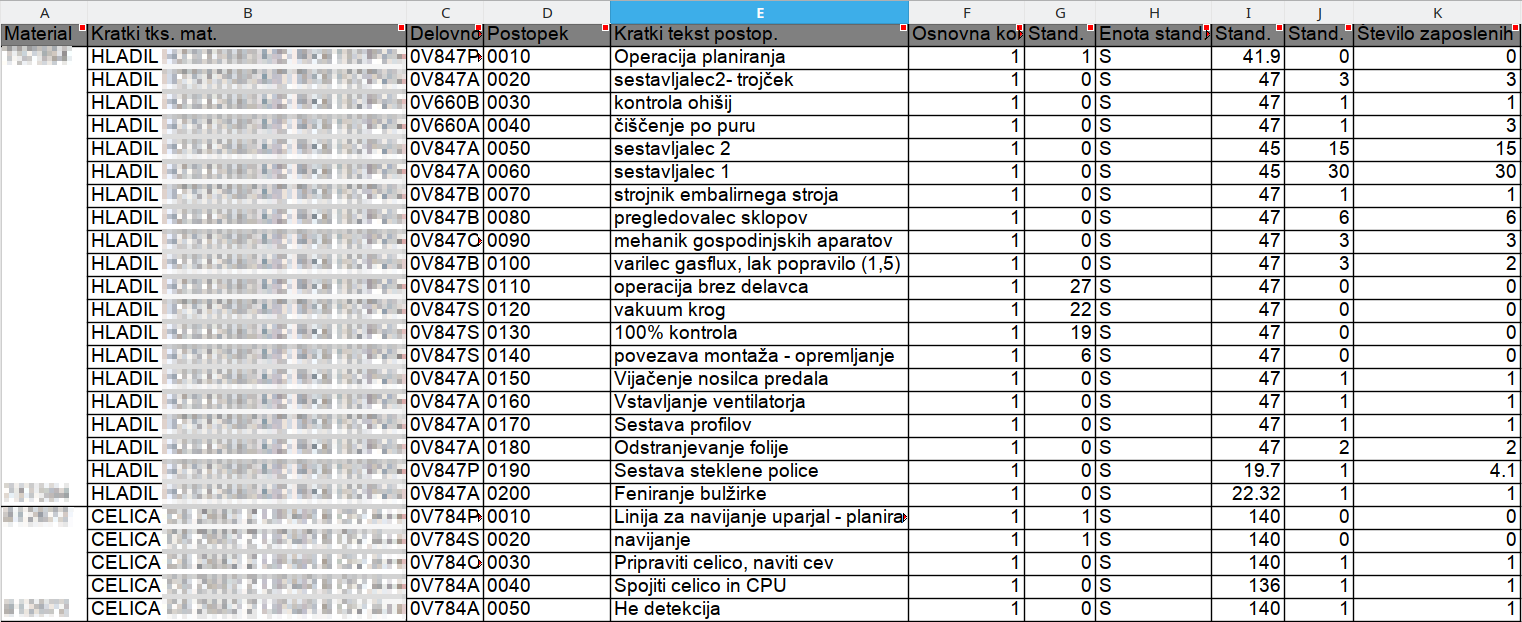
\includegraphics[width=13.5cm]{sap_2}
\end{center}
\caption{V tabelo izvožen opis tehnološkega postopka za izdelavo gospodinjskega aparata v podjetju Hisense Gorenje Europe.}
\label{sap_2}
\end{figure}

\subsection{Definicija problematike}

V diplomski nalogi raziščemo možne metode izdelave delavniškega dnevnika oz. opisa tehnološkega postopka.
Raziskati želimo prednosti in slabosti trenutnih metod sestavljanja teh dokumentov.
V naslednji fazi dela želimo izdelati specializiran sistem za sestavljanje opisov tehnoloških postopkov.
V ta sistem želimo vpeljati glasovnega pomočnika in raziskati kako uporaba glasovnega pomočnika vpliva na uporabo sistema.

\section{Funkcionalne zahteve}

Razviti želimo mobilno aplikacijo, s katero bo lahko uporabnik upravljal z zbirko delavniških dnevnikov.
Za mobilno aplikacijo smo se odločili, saj je pametni telefon veliko prikladnejši na delovnem mestu kot npr. prenosni računalnik.

Uporabniku sistema bi radi omogočili, da lahko enostavno ustvarja delavniške dnevnike in jih dodaja v svojo zbirko.
Želimo, da lahko uporabnik v delavniške dnevnike vstavlja korake, s katerimi opiše postopek dela.
Ti koraki se morajo prikazovati v preglednem in urejenem seznamu.
Za vsak delavniški dnevnik želimo imeti tudi povzetek dela in seznam možnih nevarnosti, ki pri delu pretijo delavcu.

Ker se lahko tehnološki postopki spreminjajo, želimo v delavniškem dnevniku omogočiti tudi naknadno brisanje in spreminjanje korakov.

Nekatere funkcionalnosti mobilne aplikacije želimo sprožiti prostoročno z glasovnim pomočnikom, saj bi tako sestavljalec manjkrat prekinil delo.
Med funkcionalnosti spadajo narekovanje koraka delavniškega dnevnika in odpiranje kamere za dodajanje fotografij.

Delavniške dnevnike želimo sinhronizirati na oddaljen strežnik, ki teče neodvisno od aplikacije, da se izognemo podvajanju datotek.

Uporabnik mora imeti tudi možnost izvoza svojih delavniških dnevnikov v standardne računalniške formate, ki jih lahko uporabi izven našega sistema.


\section{Uporabljene tehnologije}

\subsection{.NET}

.NET \cite{dotnet} je razvojna platforma, razvita s strani Microsofta.
Obsega programske jezike, prevajalnike, orodja in knjižnice, ki omogočajo širok spekter primerov uporabnosti, hkrati pa se ohranja enovitost ozadne kode.

Tehnologije .NET ogrodja, ki smo jih uporabil v tej diplomski nalogi, so:
\begin{itemize}
	\item .NET Core - odprtokodna platforma za razvoj spletnih storitev,
	\item Xamarin - ogrodje za razvoj mobilnih aplikacij za najpogostejše mobilne operacijske sisteme (Android, iOS).
\end{itemize}

.NET smo izbrali, ker je zelo dobro integriran z Amazonovim AWS API in je dobro dokumentiran.



\subsection{Xamarin}

Ogrodje Xamarin \cite{xamarin} je odprtokodno orodje za razvoj mobilnih aplikacij, ki ga razvija Microsoft. 

Z njim je mogoče deliti večino ozadne in ospredne kode med različnimi mobilnimi operacijskimi sistemi. 
Za ozadno kodo se uporablja .NET (C\#), za ospredno kodo pa se uporablja XAML (Extensible Application Markup Language).

Xamarin smo izbrali, da smo lahko strežniški program in mobilno aplikacijo programirali v enakem programskem jeziku (C\#).



\subsection{Amazon Alexa}

Amazon Alexa je glasovni pomočnik, razvit s strani podjetja Amazon \cite{alexa}.
Za Amazon Alexo smo se odločili, saj ponuja ogrodje za programiranje dodatnih funkcionalnosti, ki se imenuje Alexa Skills Kit.
Alexo je enostavno integrirati z drugimi Amazonovimi spletnimi storitvami, ki smo jih uporabili v tej diplomski nalogi (AWS SQS, AWS Lambda).

Alexine osnovne funkcionalnosti lahko nadgradimo s programi, ki se jim reče \enquote{Skill-i}, v nadaljevanju \enquote{veščine} (na sliki \ref{alexa_architecture}) \cite{alexaskills}.
Za razvoj in objavo Alexa veščine rabimo račun Amazon razvijalca (\textit{ang. Amazon Developer Account}).

\clearpage

\begin{figure}[H]
\begin{center}
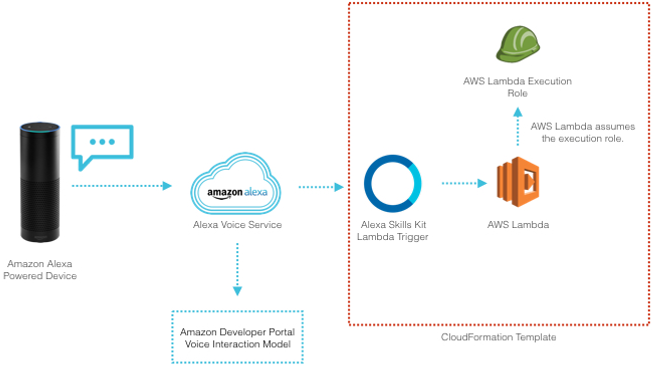
\includegraphics[width=13.5cm]{alexa_architecture}
\end{center}
	\caption{Arhitektura Alexine veščine (vir \cite{alexaarchitecture}).}
\label{alexa_architecture}
\end{figure}

\noindent Veščino sestavljajo:
\begin{itemize}
	\item \textbf{Poziv} - fraza, ki veščino zažene,
	\item \textbf{Namere} - fraze, ki jih veščina razpozna kot funkcije,
	\item \textbf{Krajišče} - omrežni vir, kjer se nahaja ozadna koda veščine.
\end{itemize}



Alexa zajame glasovni ukaz in glasovni posnetek pošlje na Amazonov Alexa Voice Service.
Ta storitev s pomočjo glasovnega razpoznavnega modela prepozna uporabnikove ukaze in pošlje poseben zahtevek na krajišče.
Krajišče je lahko druga Amazonova storitev (npr. AWS Lambda), storitev na Microsoftovem Azure strežniku, ali naš lasten strežnik, dostopen preko javne domene in zaščiten z overjenim SSL certifikatom.

Ko krajišče obdela zahtevo, odgovor pošlje nazaj na Alexa Voice Service.
Ta se iz Alexa Voice Serivice pošlje nazaj na Alexo, ki uporabniku \enquote{izgovori} prejeto sporočilo.



\subsection{Amazon Web Services}

Amazon Web Services (v nadaljevanju AWS) je skupek oblačnih storitev, ki jih ponuja podjetje Amazon.
Ponuja integracijo s pogostimi programskimi jeziki in ogrodji kot so Java, .NET, Python in Node.js preko storitve AWS API.
Pri tej diplomski nalogi smo se osredotočili na storitvi AWS Lambda in AWS Simple Queue Service.



\subsubsection{Simple Queue Service}

AWS Simple Queue Service (v nadaljevanju SQS) je sistem za pošiljanje besedilnih sporočil med odjemalci preko Amazonovih strežnikov \cite{sqs}.
To storitev smo uporabili za komunikacijo med Amazon Alexo in strežnikom implementiranega sistema.

Za hranjenje sporočil je potrebno registrirati SQS vrsto. 
Uporabili smo SQS vrsto tipa FIFO (first in, first out) \cite{sqsfifo}, pri kateri je zagotovljeno, da na strežnik prejmemo vsa sporočila v istem vrstem redu, kot so bila na SQS vrsto poslana.




\subsubsection{Lambda}

Ozadno kodo Alexa veščine smo gostili na platformi AWS Lambda, ki je storitev za gostovanje dogodkovno vodene ozadne kode \cite{lambda}.
Za to platformo smo se odločili zaradi dobre integracije z Alexa Skill Kit in razvojnim orodjem Visual Studio.




\section{Obstoječe rešitve}



\subsection{Papir in pisalo}

Najstarejša metoda za izdelavo delavniškega dnevnika je zapis na list papirja (slika \ref{paper}).

\begin{figure}[H]
\begin{center}
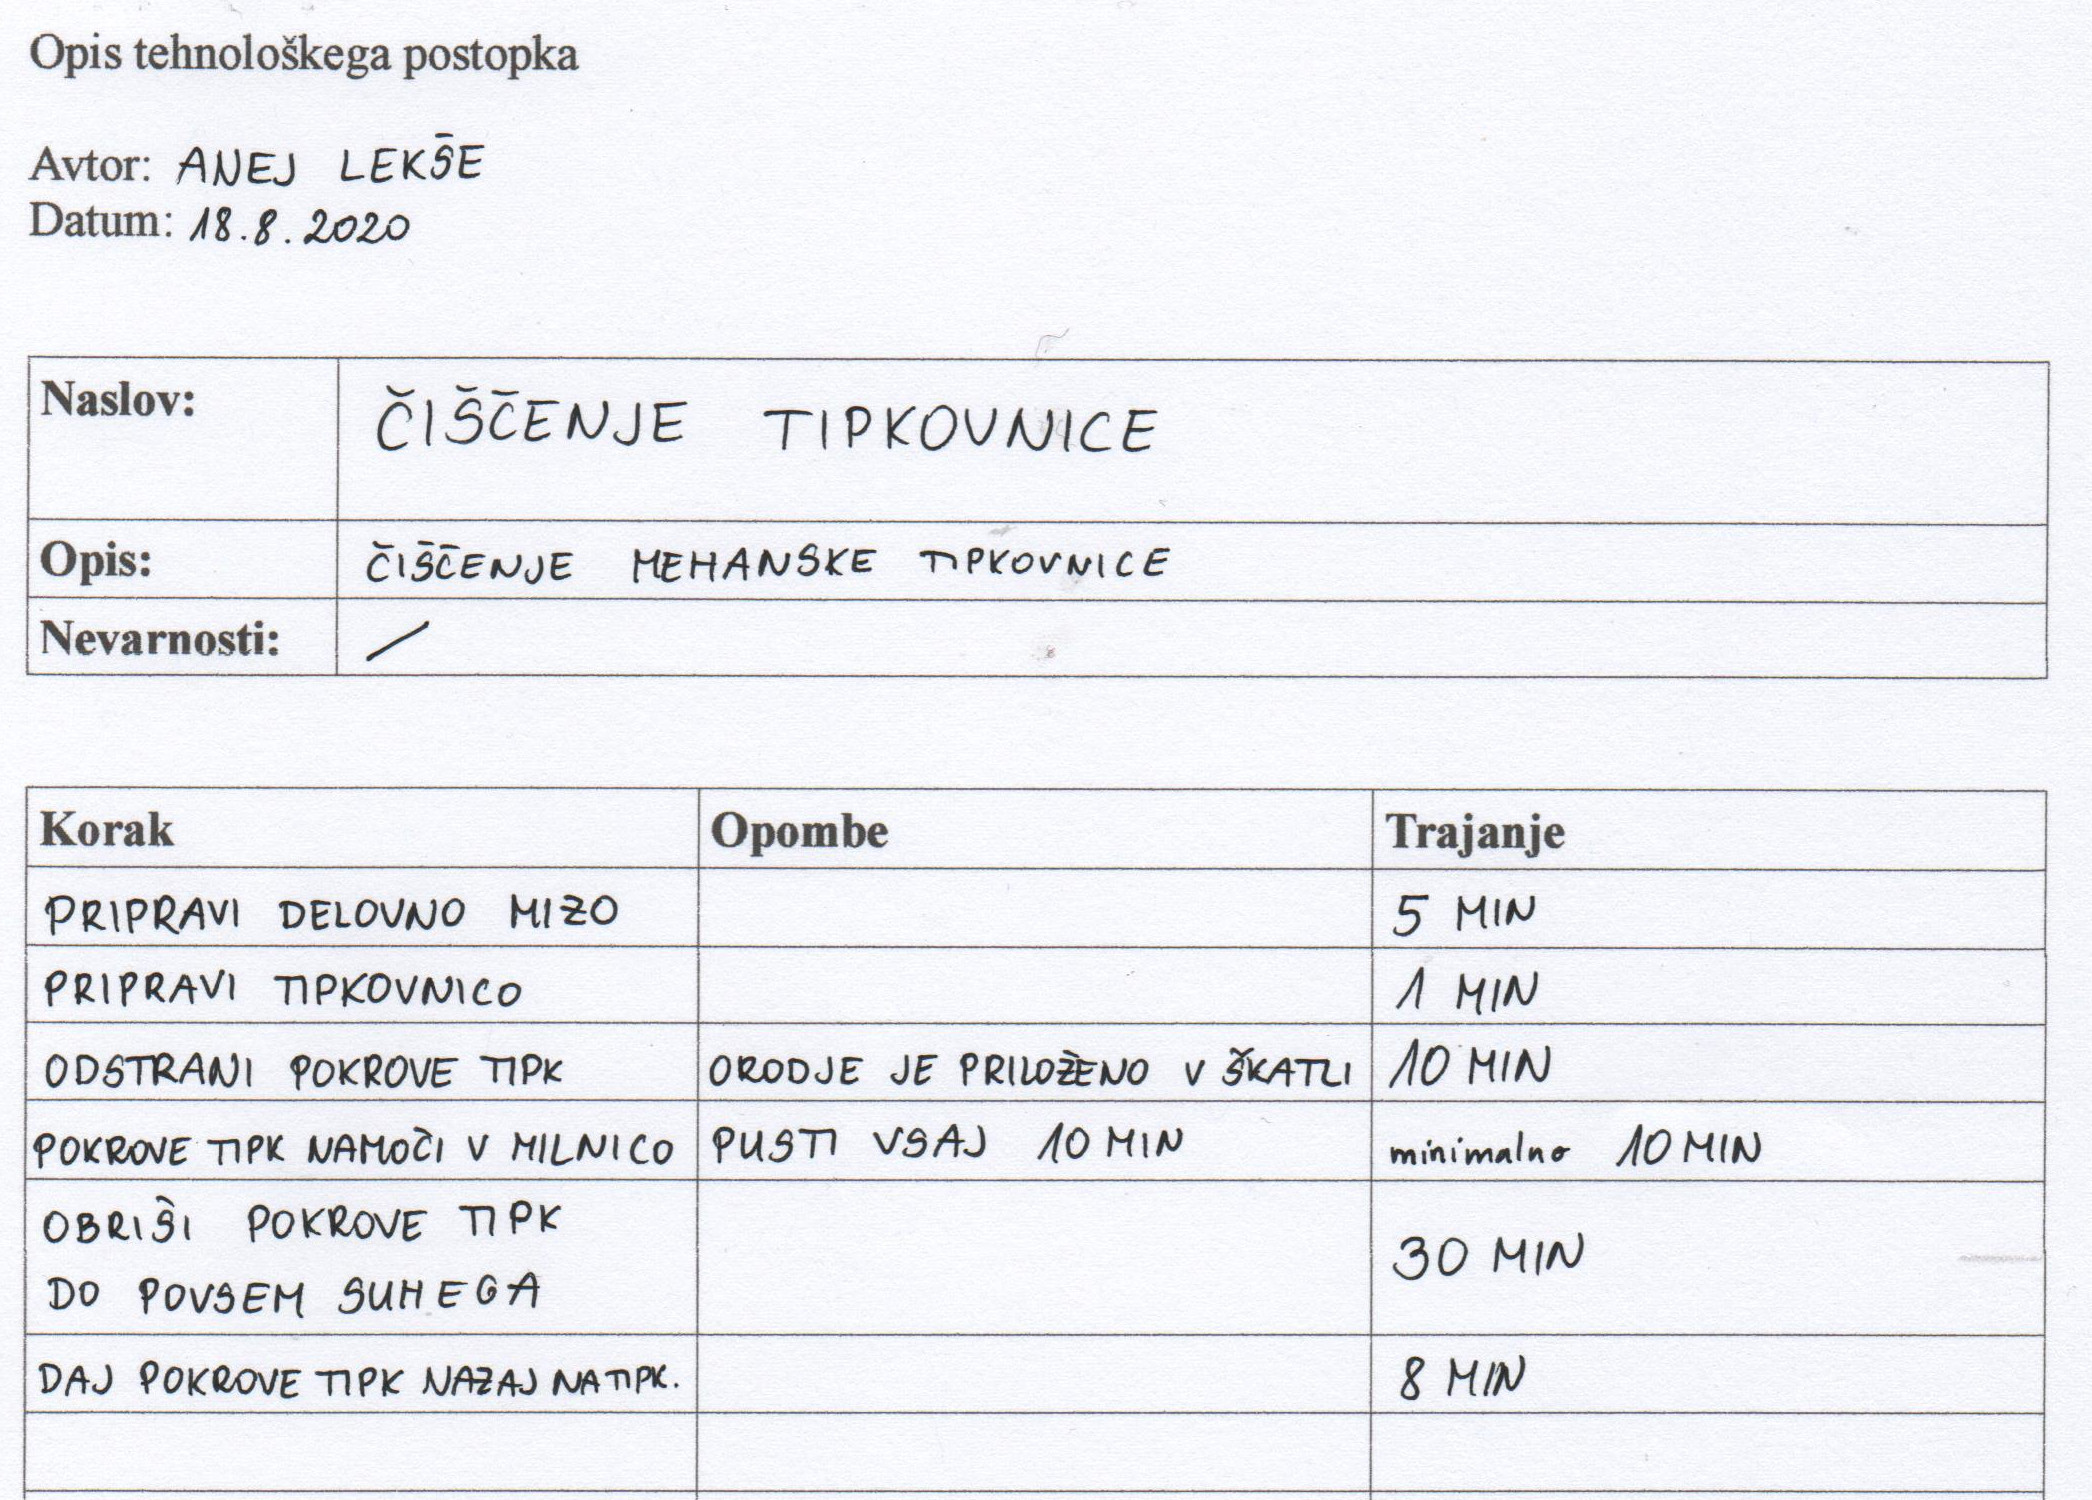
\includegraphics[width=13.5cm]{report_paper_small}
\end{center}
\caption{Opis tehnološkega postopka za čiščenje tipkovnice na papirju.}
\label{paper}
\end{figure}


\noindent Prednosti uporabe papirja in pisala pred našim sistemom so:
\begin{itemize}
	\item pri delu izdelovalec ne potrebuje računalnika in
	\item cenovna ugodnost.
\end{itemize}
V primerjavi z našim sistemom so slabosti te metode:
\begin{itemize}
	\item omejitve glede velikosti prostora, namenjenega vsakemu koraku,
	\item problematično dopisovanje in urejanje obstoječih korakov,
	\item zahtevnejše arhiviranje od računalniških datotek,
	\item občutljivost papirja na fizične poškodbe (trganje, mečkanje, vnetljivost...).
\end{itemize}



\subsection{Pisarniški programi}

Opis tehnološkega postopka lahko izdelamo v pisarniških programih, kot so na primer Microsoft Word in LibreOffice Writer.

Ta pristop reši nekatere slabosti uporabe papirja in pisala za sestavljanje opisa tehnološkega postopka.
Prednosti tega pristopa so:
\begin{itemize}
	\item enostavno dodajanje in urejanje korakov,
	\item možnost dodajanja slikovnega gradiva,
	\item pisarniški programi omogočajo izpis dokumenta na tiskalnik, če želimo imeti dokument natisnjen na papirju.
\end{itemize}

Kljub temu uporaba te metode v primerjavi z našim sistemom prinese nove slabosti:
\begin{itemize}
	\item če imamo dokument shranjen na več mestih, moramo ob spremembah zagotoviti, da se posodobijo vsi shranjeni dokumenti,
	\item slikovno gradivo je vezano na dokument; če na novo zajamemo sliko, ki smo jo vstavili v dokument, jo moramo spremeniti tudi znotraj dokumenta.
\end{itemize}

V sklopu diplomske naloge smo napisali preprost opis tehnološkega postopka (slika \ref{report_writer}) s programom LibreOffice Writer \cite{writer}.
Dokument brez vsebine se lahko pri naslednjih opisih uporabi kot obrazec za sestavljanje delavniških dnevnikov.
\clearpage

\begin{figure}[H]
\begin{center}
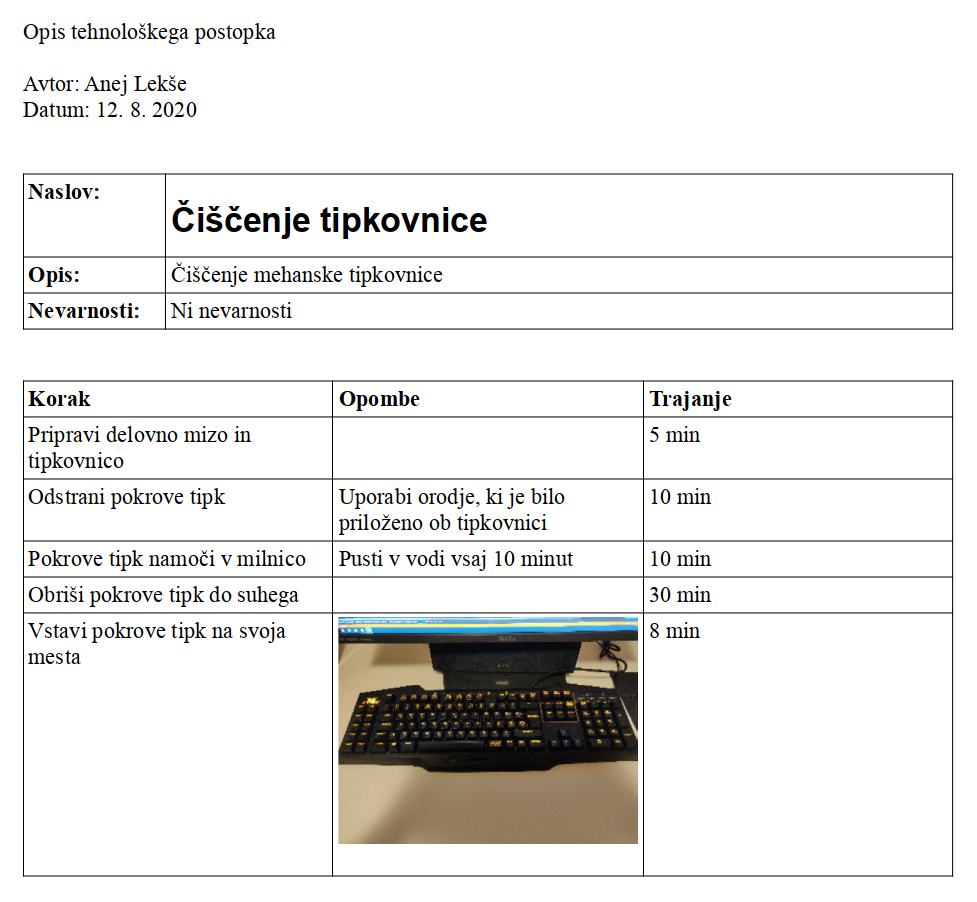
\includegraphics[width=13.5cm]{report_writer}
\end{center}
\caption{Preprost opis tehnološkega postopka za čiščenje tipkovnice, napisan v pisarniškem programu.}
\label{report_writer}
\end{figure}



\subsection{Specializirani moduli za poslovne informacijske sisteme}

Podjetja, kot so Hisense Gorenje Europe, za sestavljanje delavniških dnevnikov uporabljajo specializirane module za lastne informacijske sisteme.
Kot primer je prikazan korak opisa tehnološkega postopka v informacijskem sistemu SAP (na sliki \ref{sap_1}).

\begin{figure}[H]
\begin{center}
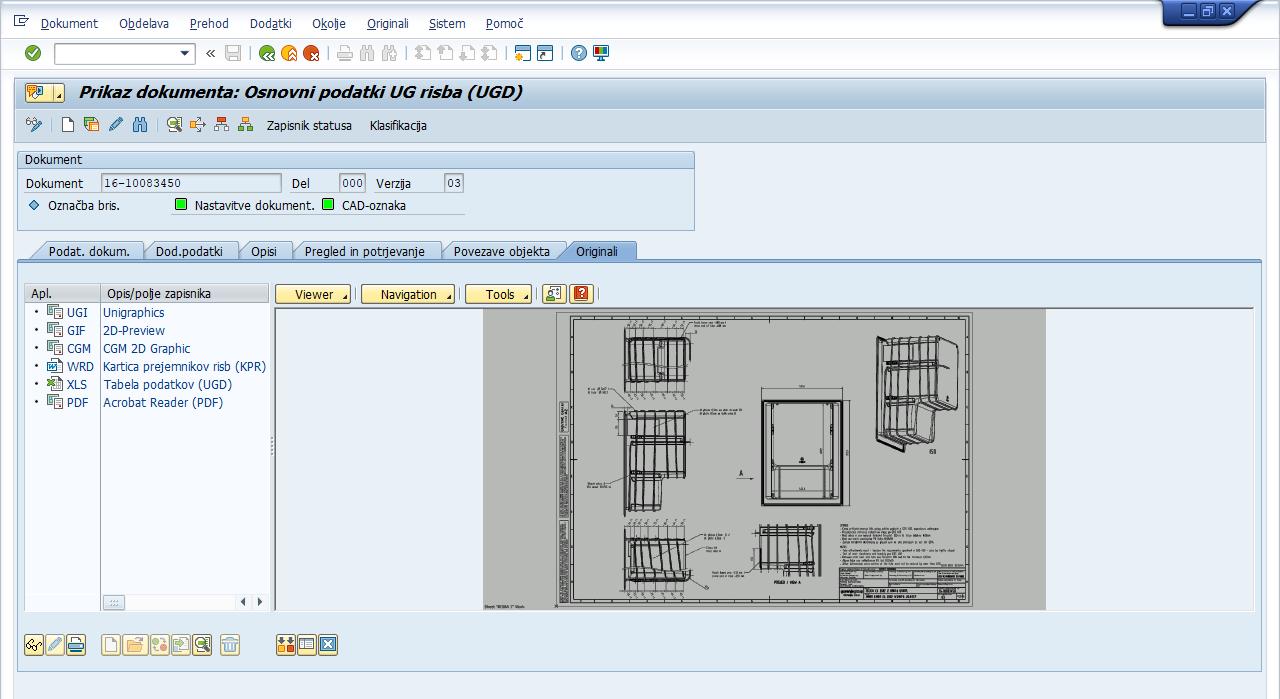
\includegraphics[width=13cm]{sap_1}
\end{center}
\caption{Prikazan korak opisa tehnološkega postopka s programom SAP.}
\label{sap_1}
\end{figure}

Do opisov tehnološkega postopka se lahko dostopa iz računalnikov na delovnih mestih.
Opis tehnološkega postopka v sistemu SAP sestavljajo:
\begin{itemize}
	\item podatki o izdelku,
	\item opisi korakov,
	\item definicija kontrolnih postopkov in pregleda, 
	\item CAD izris izdelka,
	\item dodatne opombe.
\end{itemize}

\noindent Prednosti sistema SAP pred našim sistemom so:
\begin{itemize}
	\item sistem SAP je tesno povezan s proizvodno linijo in prilagodljiv za potrebe proizvodnega obrata, ki ga uporablja,
	\item podatki se hranijo na osrednjem strežniku, varnostna kopija pa se inkrementalno dela na geografsko ločen rezervni strežnik.
\end{itemize}

Takšni sistemi predstavljajo v primerjavi z našim naslednje slabosti:
\begin{itemize}
	\item zahtevajo dovršeno proizvodno infrastrukturo, ki jo sistem rabi za optimalen izkoristek in
	\item visoka cena, ki je potrebna za implementacijo takega sistema v proizvodno linijo.
\end{itemize}




\chapter{Načrtovanje in razvoj sistema}



\section{Definicija funkcionalnosti} \label{architecture}

Sistem, ki smo ga v sklopu diplomske naloge implementirali (na sliki \ref{plan_simple}), uporabniku omogoča vodenje svojih delavniških dnevnikov (v nadaljevanju imenovanih tudi \textit{projektov}).
Služil bo kot alternativa pisanju delavniških dnevnikov s pisarniškimi programi.
Vsak projekt ima zbirko \textit{korakov}.
Korak opisuje posmezno dejavnost tehnološkega postopka, ki ga želimo zabeležiti z delavniškim dnevnikom.

Implementiran sistem sestavljajo:
\begin{itemize}
	\item mobilna aplikacija,
	\item glasovni pomočnik in
	\item strežnik.
\end{itemize}

\clearpage

\begin{figure}[H]
\begin{center}
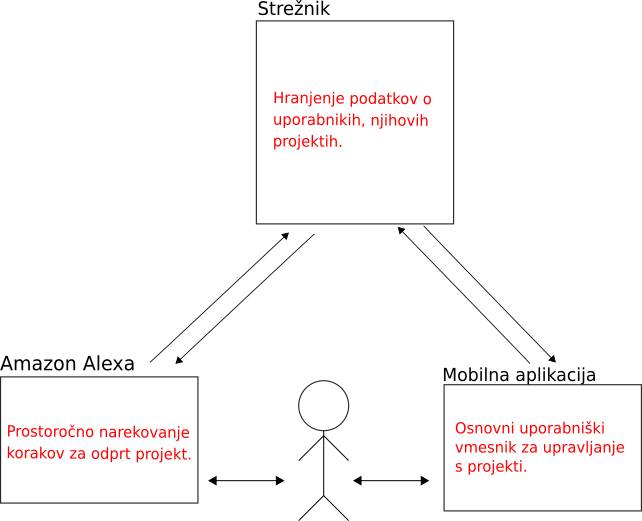
\includegraphics[width=13cm]{plan_simple}
\end{center}
\caption{Arhitektura sistema.}
\label{plan_simple}
\end{figure}


Osnovni uporabniški vmesnik sistema je mobilna aplikacija.
Z aplikacijo se uporabnik prijavi v sistem s svojim uporabniškim računom, ustvarja, odpira in ureja svoje delavniške dnevnike.

Delavniški dnevnik oz. projekt sestavljajo naslov, opis dela, opis možnih nevarnosti in seznam korakov postopka.
Korake sestavljajo naslov, opis in predvideno trajanje koraka.

% V odprt projekt lahko uporabnik dodaja korake, ki opisujejo potek dela.
Seznam korakov postopka mora podpirati dodajanje novih korakov, posodabljanje vsebine obstoječih korakov, brisanje obstoječih korakov in spreminjanje vrstnega reda korakov.
Uporabnik lahko tudi posname fotografije in jih doda v odprt projekt kot korak.
Vsi podatki, ki jih uporabnik vnese preko mobilne aplikacije in glasovnega pomočnika, se hranijo na strežniku.

Glasovnega pomočnika smo uporabili kot razširitev uporabniškega vmesnika.
Z implementacijo glasovnega pomočnika smo želeli doseči:
\begin{itemize}
	\item prostoročno narekovnaje besedilnega koraka projekta,
	\item prostoročno odpiranje obrazca za dodajanje koraka v projekt in
	\item prostoročno odpiranje kamere na mobilni napravi.
\end{itemize}


% Opredeljeno natančneje, sistem mora uporabniku omogočati ustvarjanje novega opisa tehnološkega postopka in odpiranje ter urejanje obstoječih opisov tehnološkega postopka.
 
% Vsak ustvarjen opis tehnološkega postopka mora imeti naslov, opis dela, opis možnih nevarnosti pri delu in seznam korakov dela, ki ga sestavljajo.
 
 
% Posamezen korak mora imeti naslov, opis dela in predvideno trajanje opisanega dela.





\subsection{Izboljšave z glasovnim pomočnikom}

% Glasovni pomočnik v našem sistemu služi kot uporabniški vmesnik za prostoročno dodajanje korakov v odprt projekt.
% DELJENJE
Komunikacija z glasovnim pomočnikom je smiseln način interakcije z računal-\\niškim sistemom v situaciji, kjer uporabnik nima prostih rok ali je fizično oddaljen od naprave.
% Osnovna funkcionalnost glasovnega pomočnika je prostoročno narekovanje besedila koraka v projektu.
% Implementirali smo tudi odpiranje obrazcev za dodajanje korakov v projekt in zagon kamere.

% \bigbreak 
% Glasovni pomočnik v našem sistemu ima naslednje vloge:
% \begin{itemize}
% 	\item za trenutno odprt opis tehnološkega postopka je z njim možno dodajati korake postopka,
% 	\item z njim je možno odpreti kamero ali obrazec za dodajanje koraka.
% \end{itemize}

Raziskava iz leta 2018 \cite{austerjost2018introducing} je pokazala izboljšano učinkovitost pri delu raziskovalcev v kemijskem laboratoriju, v katerega so integrirali glasovne pomočnike.
Namen raziskave je bil preizkus praktične uporabnosti glasovnih pomočnikov za branje laboratorijskih postopkov in glasovno upravljanje laboratorijskih instrumentov.
Pozitivni rezultati bi lahko bili ključnega pomena za slabovidne člane laboratorijev.
Kot glasovnega pomočnika so uporabili Amazon Alexo.
Prepoznavanje govora in ukazov je bilo konsistentno in hitro, ne glede na spol uporabnika.
Motnje pri razpoznavanju je povzročal večinoma hrup v ozadju.
Povprečna uspešnost prepoznave ukazov je bila 95\%.
% Raziskovalci so zabeležili tudi problem moteče kakofonije v laboratoriju, v katerem je več raziskovalcev, ki uporabljajo glasovni nadzor naprav.




\section{Načrt sistema za sestavljanje opisov tehnoloških postopkov}

Implementirali smo arhitekturo, ki je predstavljena v poglavju \ref{architecture}.
Sistem smo poimenovali OpenReport (na sliki \ref{plan}), ki ga sestavljajo:
\begin{itemize}
	\item mobilna aplikacija,
	\item strežniški program in 
	\item Amazon Alexa.
\end{itemize}

\begin{figure}[H]
\begin{center}
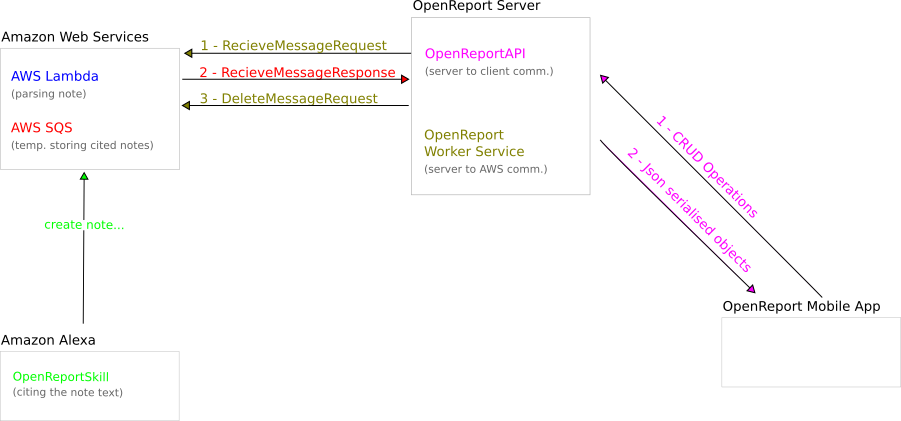
\includegraphics[width=13cm]{plan}
\end{center}
\caption{Visokonivojski načrt sistema.}
\label{plan}
\end{figure}

Strežnik v podatkovni bazi hrani uporabniške račune in opise tehnoloških postopkov.
Uporabnik lahko do podatkov dostopa preko mobilne aplikacije, ki s strežnikom komunicira preko API.
Glasovnega pomočnika smo uporabili kot dodatek k mobilni aplikaciji.
Omogoča glasovno upravljanje aplikacije in narekovanje korakov.

\bigbreak
Preko mobilne aplikacije uporabnik lahko:
\begin{itemize}
	\item opravi regsitracijo in prijavo,
	\item ustvari nov delavniški dnevnik,
	\item odpre obstoječe delavniške dnevnike,
	\item ustvarja in ureja korake delavniškega dnevnika,
	\item zajema slike in jih vstavlja v delavniški dnevnik,
	\item briše korake delavniškega dnevnika,
	\item ureja vrstni red korakov delavniškega dnevnika.
\end{itemize}

Za glasovnega pomočnika Amazon Alexa smo razvili veščino, s katerim uporabnik lahko:

\begin{itemize}
	\item v odprto poročilo vstavi dobesedno narekovan korak,
	\item odpre obrazec za dodajanje novega besedilnega koraka,
	\item odpre kamero in obrazec za dodajanje koraka s fotografijo.
\end{itemize}



\section{Strežnik}

Osrednja komponenta sistema OpenReport je strežnik.
Zadolžen je za delo s podatki uporabnikov in delavniškimi dnevniki.
Odjemalci, ki so nanj povezani, služijo zgolj kot \enquote{uporabniški vmesnik} za zajem in prikaz podatkov na strežniku.

% Operacije s podatki, hranjenimi na strežniku, se sprožijo na strani odjemalca in izvedejo na strežniku.

\noindent Osnovne naloge strežnika so:
\begin{itemize}
	\item avtentikacija uporabnikov,
	\item avtorizacija uporabnikovih zahtev,
	\item komunikacija z glasovnim pomočnikom,
	\item hranjenje podatkov o uporabnikih in delavniških dnevnikih, 
	\item ponujanje vmesnika, ki ga lahko odjemalci uporabijo za operacije nad delavniškimi dnevniki.
\end{itemize}

Podatke hranimo na strežniku, da lahko do podatkov dostopamo iz različnih naprav preko enotnega vmesnika.
To nam omogoča enostavno dodajanje odjemalcev in odpravi podvajanje podatkov med napravami.

S strežnikom komunicirata mobilna aplikacija in glasovni pomočnik.
Podatke hranimo v podatkovni bazi, ki jo hrani SQL Server.



\subsection{Komunikacija z odjemalci}

Strežnik z odjemalci komunicira preko API zaradi enostavnosti implementacije in možnosti širjenja nabora odjemalcev v prihodnosti.

V našem primeru je bil osnovni odjemalec mobilna aplikacija.
Odjemalec na definirane funkcijske URL-je (slika \ref{api_routes}) strežnika pošlje HTTP zahtevke.
Če so zahtevki pravilno oblikovani, strežnik izvede predvideno funkcijo in rezultat te funkcije pošlje kot HTTP odgovor nazaj odjemalcu.
Komunikacija med strežnikom in odjemalcem je prikazana z roza barvo na sliki \ref{plan_server_client}.

\clearpage

\begin{figure}[H]
\begin{center}
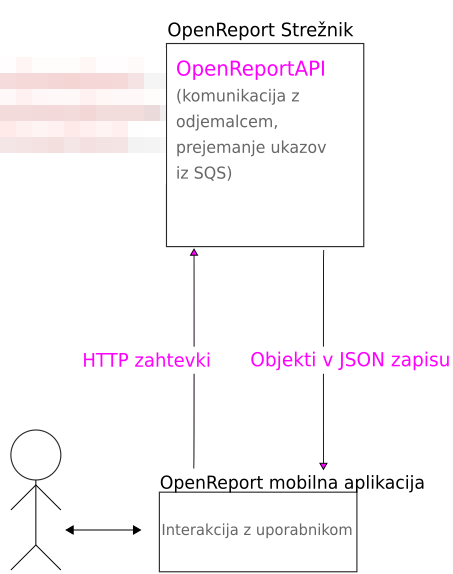
\includegraphics[width=8cm]{plan_server_client}
\end{center}
\caption{Komunikacija strežnika z odjemalcem.}
\label{plan_server_client}
\end{figure}


\subsection{Podatkovni model}

Podatke smo razdelili v tri entitete:
\begin{itemize}
	\item uporabnik,
	\item delavniški dnevnik,
	\item korak delavniškega dnevnika.
\end{itemize}

Uporabnik lahko sestavlja svoje delavniške dnevnike, vsak delavniški dnevnik pa je sestavljen iz zbirke korakov.

Podatkovna baza hrani tabele \enquote{AspNetUsers}, \enquote{Projects} in \enquote{Notes} (slika \ref{er_diagram}).
Vsak uporabnik lahko ima 0 ali mnogo delavniških dnevnikov.
Vsak projekt ima lahko 0 ali mnogo korakov.

\begin{figure}[H]
\begin{center}
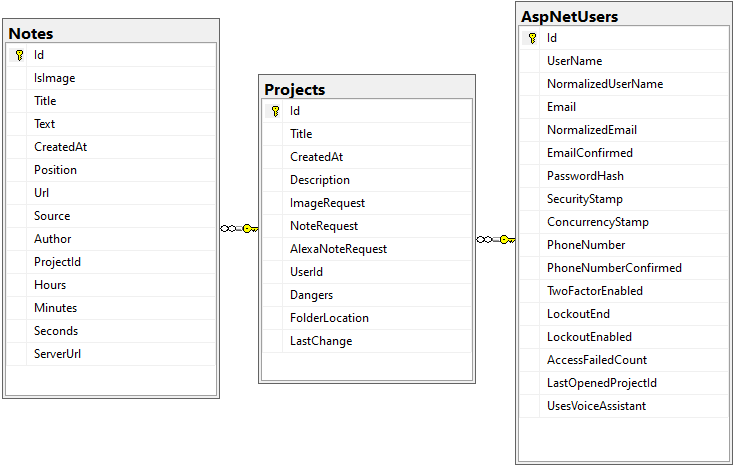
\includegraphics[width=13.5cm]{er_diagram_small}
\end{center}
\caption{ER model podatkovne baze.}
\label{er_diagram}
\end{figure}

Uporabnik ima uporabniško ime, katerega uporabi za prijavo, in geslo s katerim dokaže, da je to res on.
% Uporabnik mora imeti možnost dodajanja svojih projektov.

Vsak delavniški dnevnik ima naslov, opis in enolični identifikator uporabnika, ki si dnevnik lasti.

Vsak korak delavniškega dnevnika ima naslov, opis, podatke o trajanju in enolični identifikator projekta, ki si korak lasti.




\section{Implementacija strežnika in mobilne aplikacije}

Komunikacija med odjemalcem in strežnikom poteka preko spletnega API (slika \ref{api_routes}), ki ga ponuja strežnik.

Ker lahko sistem uporablja več uporabnikov, smo implementirali sistema za avtentikacijo uporabnikov in avtorizacijo zahtev.
Avtentikacija z uporabniškim imenom in geslom omogoča preverjanje identitete.
Ko se vzpostavi zaupanje, se uporabniku dodeli avtorizacijski žeton.


\begin{figure}[H]
\begin{center}
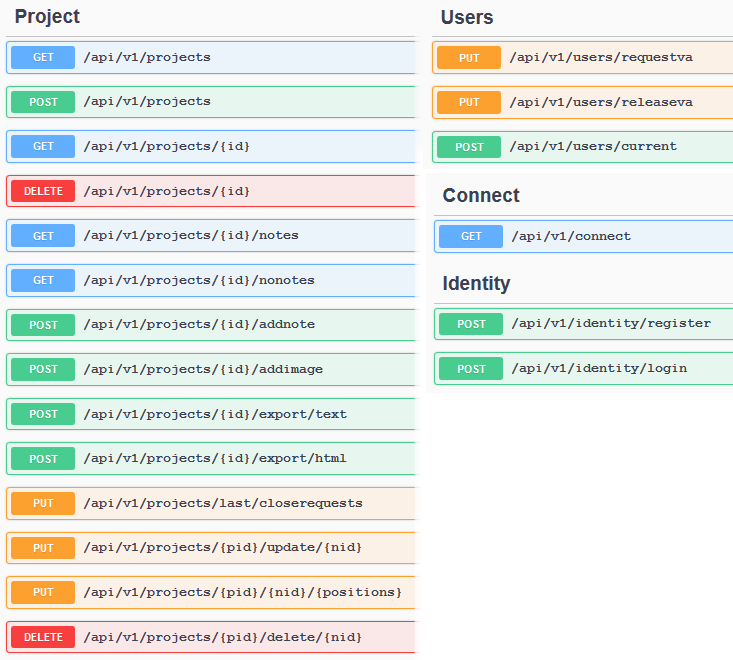
\includegraphics[width=13.5cm]{api_routes_small}
\end{center}
\caption{Seznam razvitih in dokumentiranih API funkcij.}
\label{api_routes}
\end{figure}

\subsection{Pristop razvoja mobilne aplikacije}

Pristop razvoja aplikacije, ki smo ga uporabili za programiranje aplikacije, se imenuje \enquote{Model View View-Model} (v nadaljevanju MVVM).
Pri tem pristopu aplikacijo razdelimo na tri dele (slika \ref{mvvm}).

V \textbf{Modelu} definiramo elemente naše podatkovne logike (opis tehnološkega postopka, korak, uporabnik).

\textbf{View} je uporabniški vmesnik, ki ga vidi uporabnik.

\textbf{View-Model} pa se uporablja, da se poveže funkcije uporabniškega vmesnika in podatkovne logike, ter po potrebi preoblikuje podatke.

Rezultat upoštevanja tega pristopa je čista koda, ki nima prepletenih elementov med ozadno kodo in uporabniškim vmesnikom.
\enquote{Model} vsebuje le abstrakcijo naših podatkov in podatkovno logiko.
Ti podatki se v \enquote{ViewModel-u} pretvorijo v obliko, ki bo prikazana uporabniku.
\enquote{View} nato prikaže pripravljene podatke uporabniku v obliki grafičnih elementov.

Na spodnji sliki lahko vidimo oris pristopa MVVM (slika \ref{mvvm}).

\begin{figure}[H]
\begin{center}
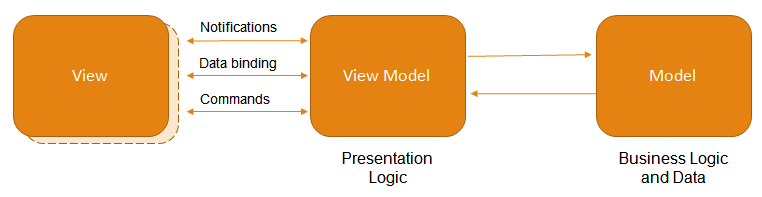
\includegraphics[width=11cm]{mvvm}
\end{center}
	\caption{Shema pristopa MVVM (vir \cite{mvvmimage}).}
\label{mvvm}
\end{figure}


\subsection{Registracija in prijava}

Vse operacije nad uporabnikovimi delavniškimi dnevniki morajo biti avtorizirane, zato mora uporabnik vzpostaviti zaupanje s strežnikom.
To uporabnik stori tako, da se v sistem prijavi s svojim uporabniškim imenom in geslom.
Ob prvi uporabi se mora uporabnik registrirati (slika \ref{app_register}).

Ob uspešni avtentikaciji uporabnik od strežnika prejme avtorizacijski žeton, ki mu dovoljuje dostop do njegovih delavniških dnevnikov.
Aplikacija doda avtorizacijski žeton vsem nadaljnjim HTTP zahtevkom na strežnik.


\begin{figure}[H]
\begin{center}
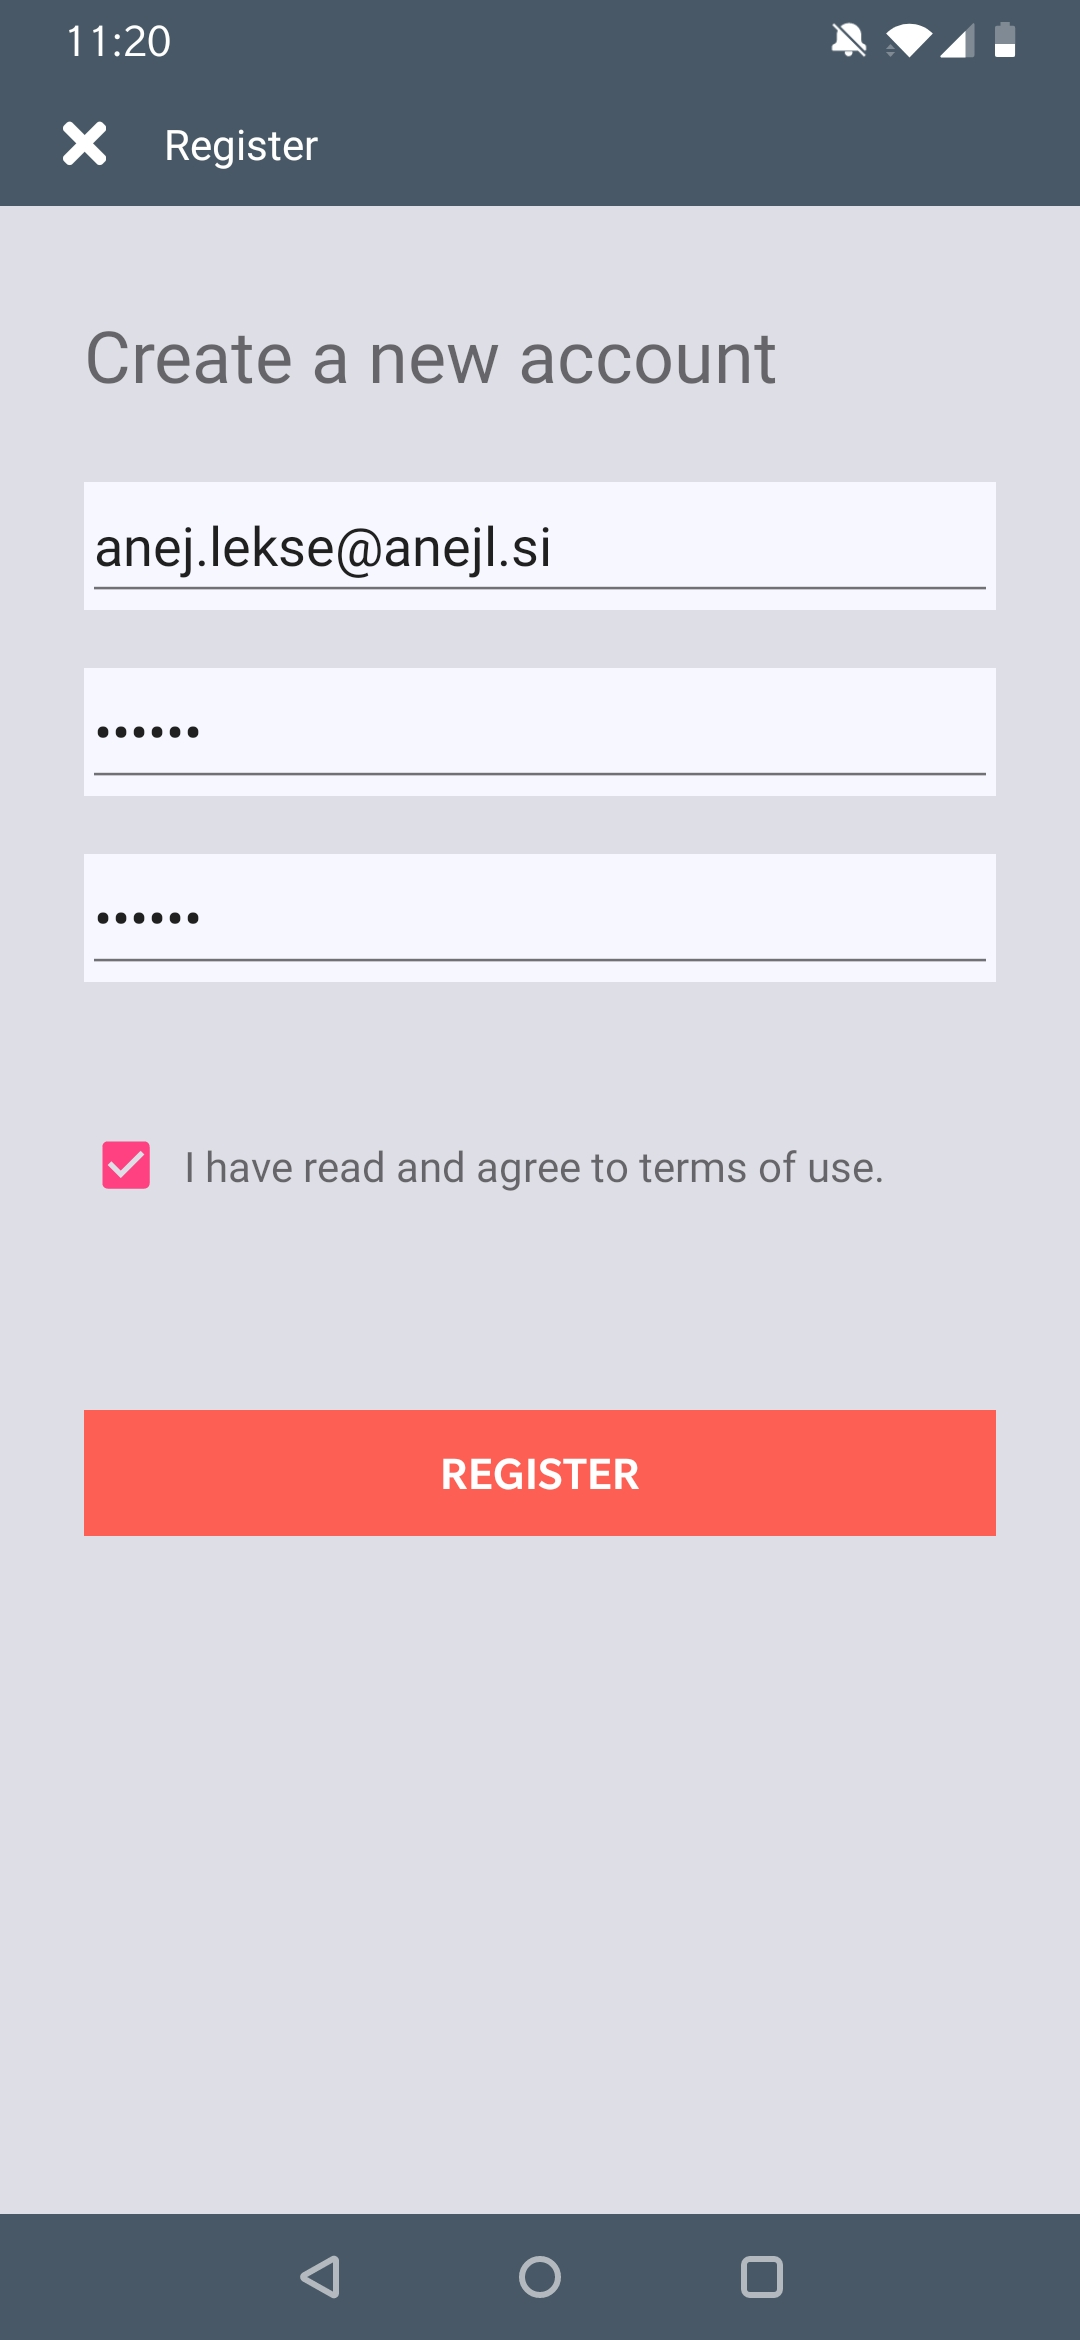
\includegraphics[width=6cm]{app_register}
\end{center}
	\caption{Registracijska stran v mobilni aplikaciji.}
\label{app_register}
\end{figure}

Pri registraciji mobilna aplikacija na strežnik pošlje objekt razreda \texttt{Regis-\\terUserRequest} na URL \enquote{\texttt{/identity/register}} preko metode POST.
V objektu \texttt{RegisterUserRequest} se nahajata njegov e-mail naslov in geslo v čisti obliki.

\begin{verbatim}
RegisterUserRequest {
    string Email; 
    string Password; 
} 
\end{verbatim}


Na strežniku zahtevek obdela avtentikacijska storitev.
Storitev preveri, ali je e-naslov v polju \texttt{Email} že bil registriran.
Če je bil, se zabeleži napaka in nadaljnja registracija se prekine.
Če ta uporabnik ne obstaja, se ustvari nov objekt razreda \texttt{User}.
Polje \texttt{Password} se šifrira in se skupaj s poljem \texttt{Email} zapiše v ta objekt.
Objekt se zapiše v podatkovno bazo v tabelo \texttt{Users}.
Uporabnik pri registraciji dobi tudi svoj enoličen identifikator \texttt{Id}.

Objekt \texttt{AuthFailedResponse} se vrne odjemalcu ob napaki med avtentikacijo.
Vsebuje seznam vseh zabeleženih napak.

\begin{verbatim}
AuthFailedResponse { 
     IEnumerable<string> Errors; 
}
\end{verbatim}

Objekt razreda \texttt{AuthSuccessResponse} se pošlje odjemalcu ob uspešni registraciji.

\begin{verbatim}
AuthSuccessResponse { 
    string UserId; 
    string Token; 
} 
\end{verbatim}

V polje \texttt{Token} razreda \texttt{AuthSuccessResponse} se zapiše avtorizacijski žeton.
Žeton je tipa JWT ali \texttt{JSON Web Token} \cite{jwtinfo}.
Sestavljajo ga e-mail uporabnika, uporabnikov enolični identifikator, čas zapada žetona in tip simetričnega šifriranja, uporabljenega za šifriranje žetona.

Žeton v objektu razreda \texttt{AuthSuccessResponse} se pošlje odjemalcu.
% Strežnik ga uporabi pri poizvedbah po podatkovni bazi.

\clearpage

\begin{figure}[H]
\begin{center}
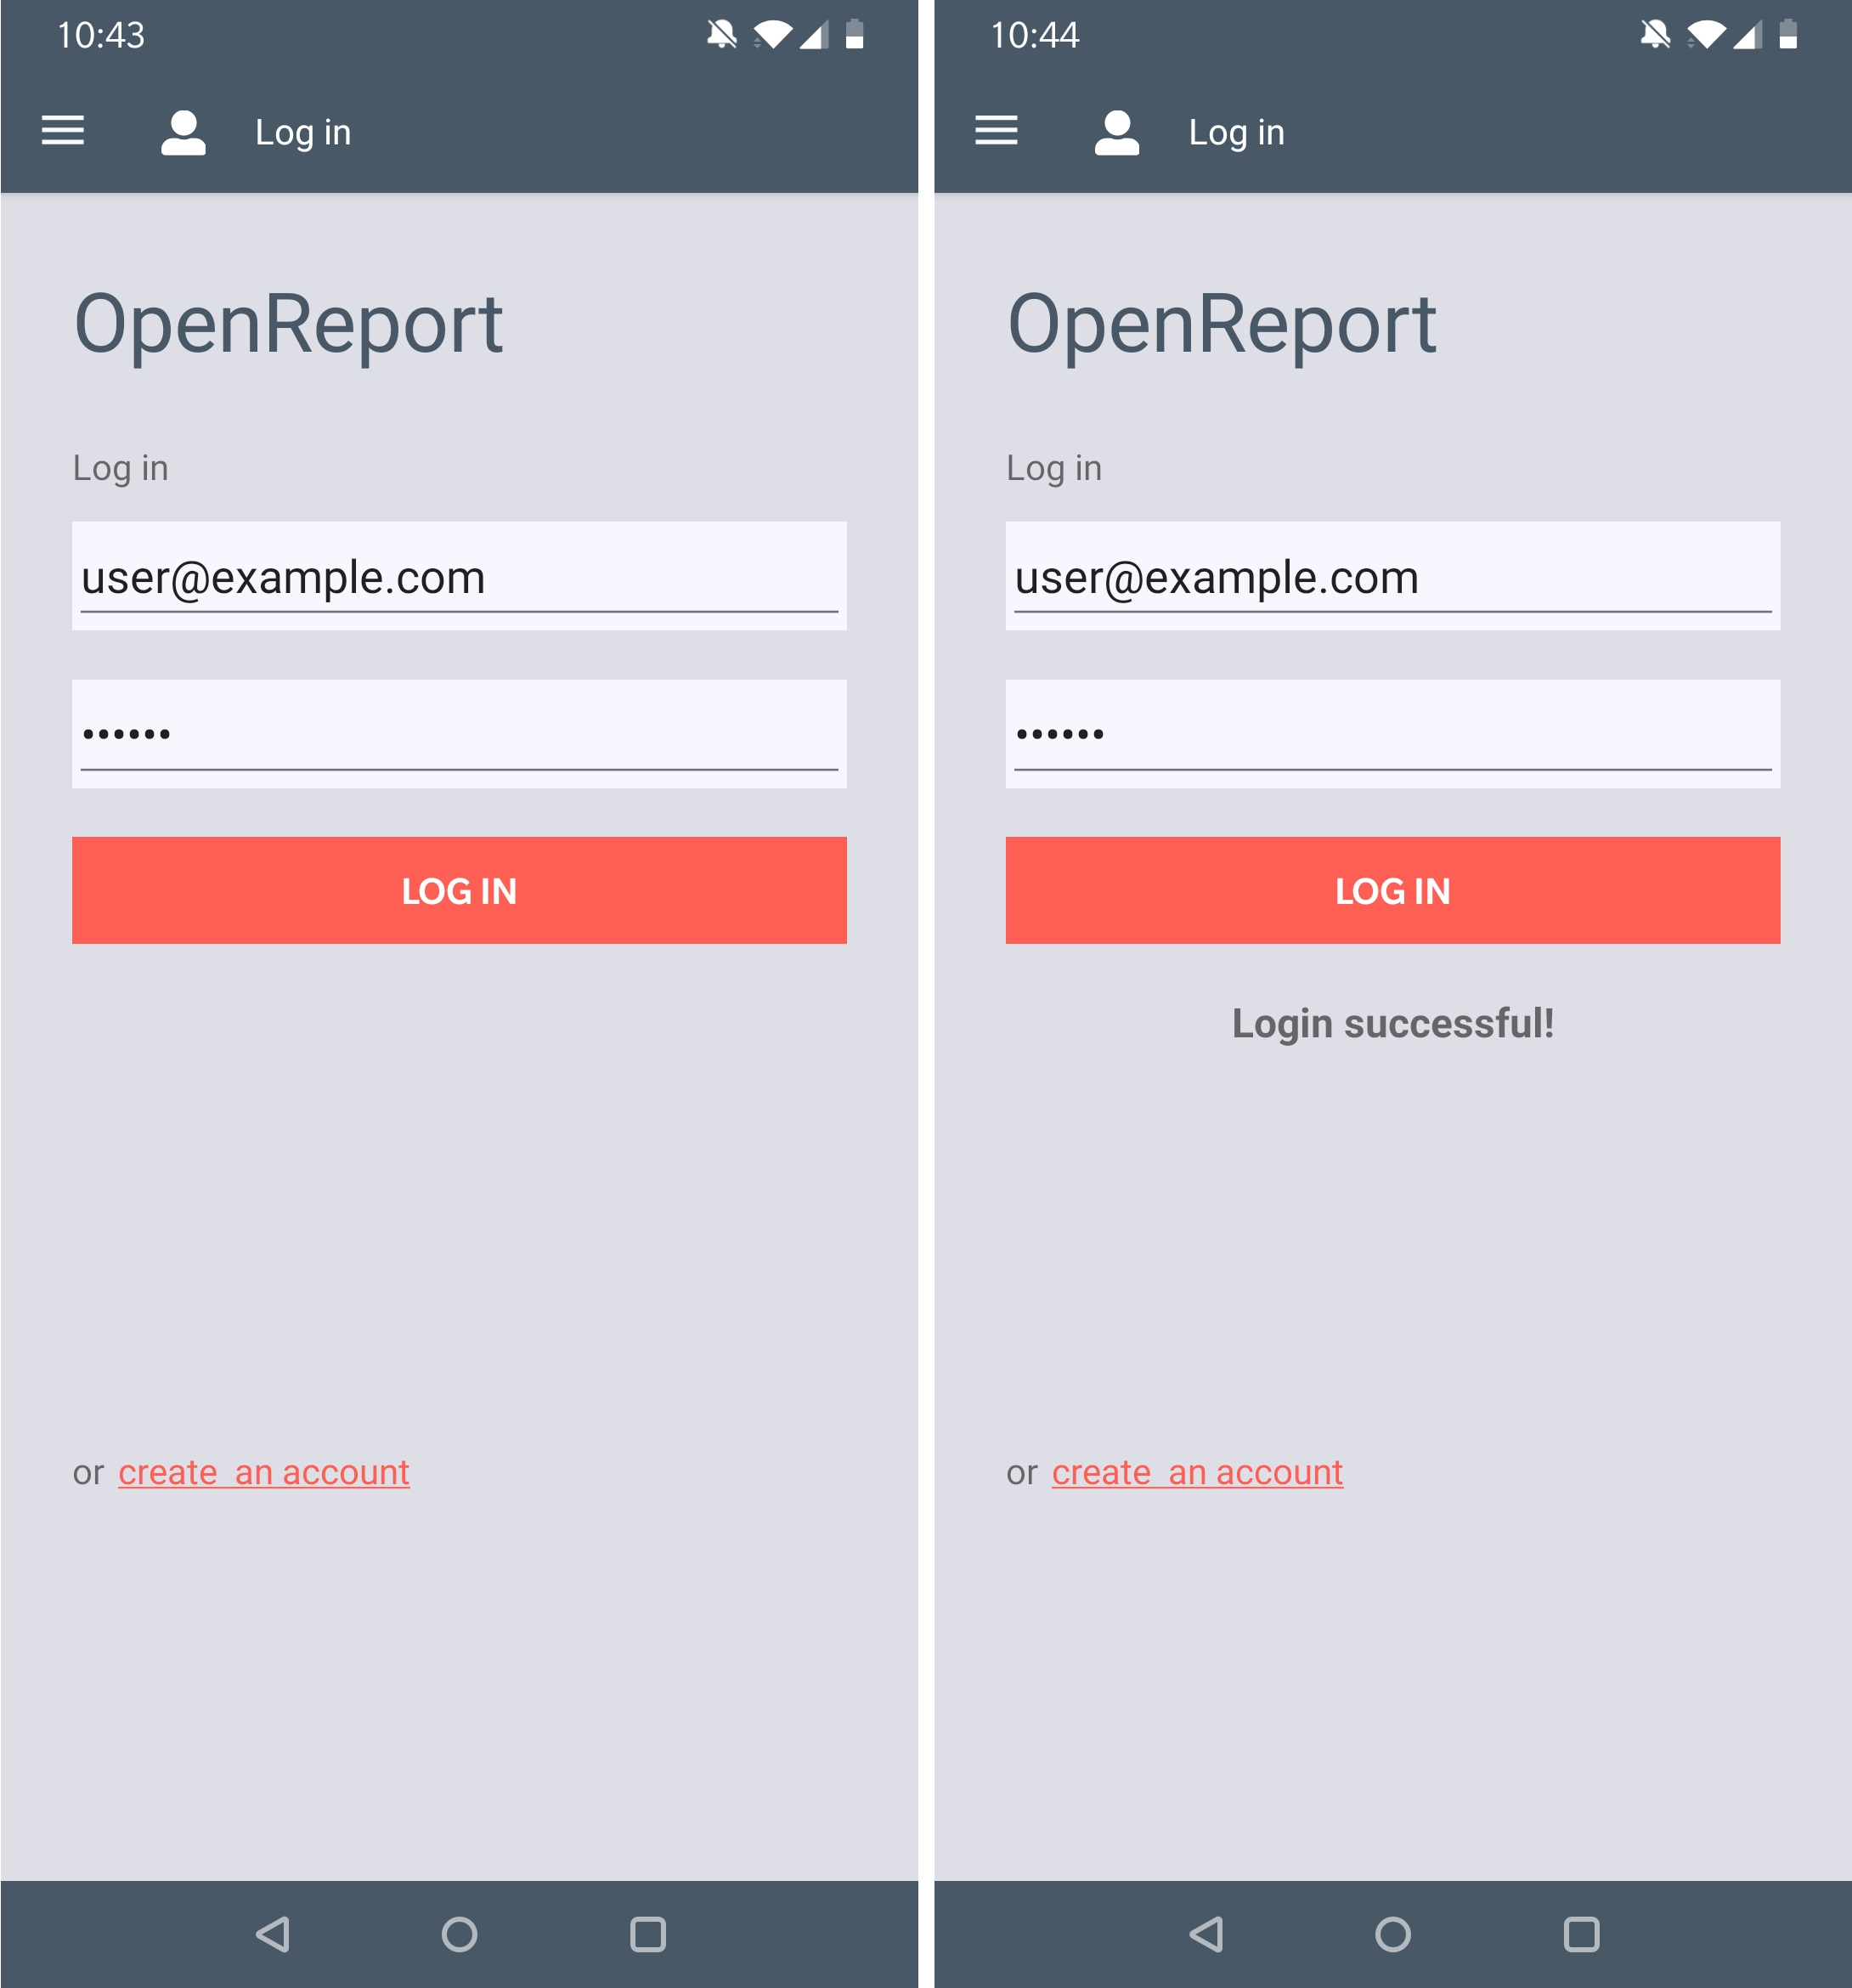
\includegraphics[width=8cm]{app_login}
\end{center}
	\caption{Prijavna stran pred poskusom prijave (levo), in po uspešnem poskusu prijave (desno).}
\label{app_login}
\end{figure}

Prijava (na sliki \ref{app_login}) poteka podobno.
Odjemalec na strežnik pošlje objekt razreda \texttt{LoginUserRequest} na URL \enquote{\texttt{/identity/login}}.
Objekt \texttt{LoginUserRequest} vsebuje e-mail naslov in geslo v čisti obliki.

\begin{verbatim}
LoginUserRequest {
    string Email; 
    string Password; 
} 
\end{verbatim}

Avtentikacijska storitev preveri, ali uporabnik s tem e-naslovom že obstaja.
Če uporabnik ne obstaja ali pa je šifrirano geslo v podatkovni bazi drugačno kot to, kar je v polju \texttt{Password}, zabeležimo napake in prijava se prekine.
Strežnik odjemalcu pošlje objekt razreda \texttt{AuthFailedResponse} s seznamom napak.

Če uporabnik s podanim e-naslovom obstaja in se šifrirano geslo iz polja \texttt{Password} ujema z geslom v podatkovni bazi, strežnik odjemalcu pošlje avtorizacijski žeton v objektu razreda \texttt{AuthSuccessResponse}.

% Storitev za komunikacijo s strežnikom v mobilni aplikaciji prejet žeton doda glavi vseh svojih nadaljnjih zahtevkov na strežnik.



\subsection{Operacije z delavniškimi dnevniki}

Po prijavi lahko uporabnik odpre stran s seznamom njegovih delavniških dnevnikov, imenovano Dashboard (na sliki \ref{app_dashboard_first}).
Na tej strani se prikažejo:
\begin{itemize}
	\item seznam vseh njegovih projektov, 
	\item gumbi za izbris posameznega projekta,
	\item gumb za dodajanje novega projekta, 
	\item gumb za zahtevanje in sprostitev glasovnega pomočnika.
\end{itemize}

% Sistem omogoča dodajanje, odpiranje in brisanje delavniških dnevnikov prijavljenemu uporabniku.

\clearpage

\begin{figure}[H]
\begin{center}
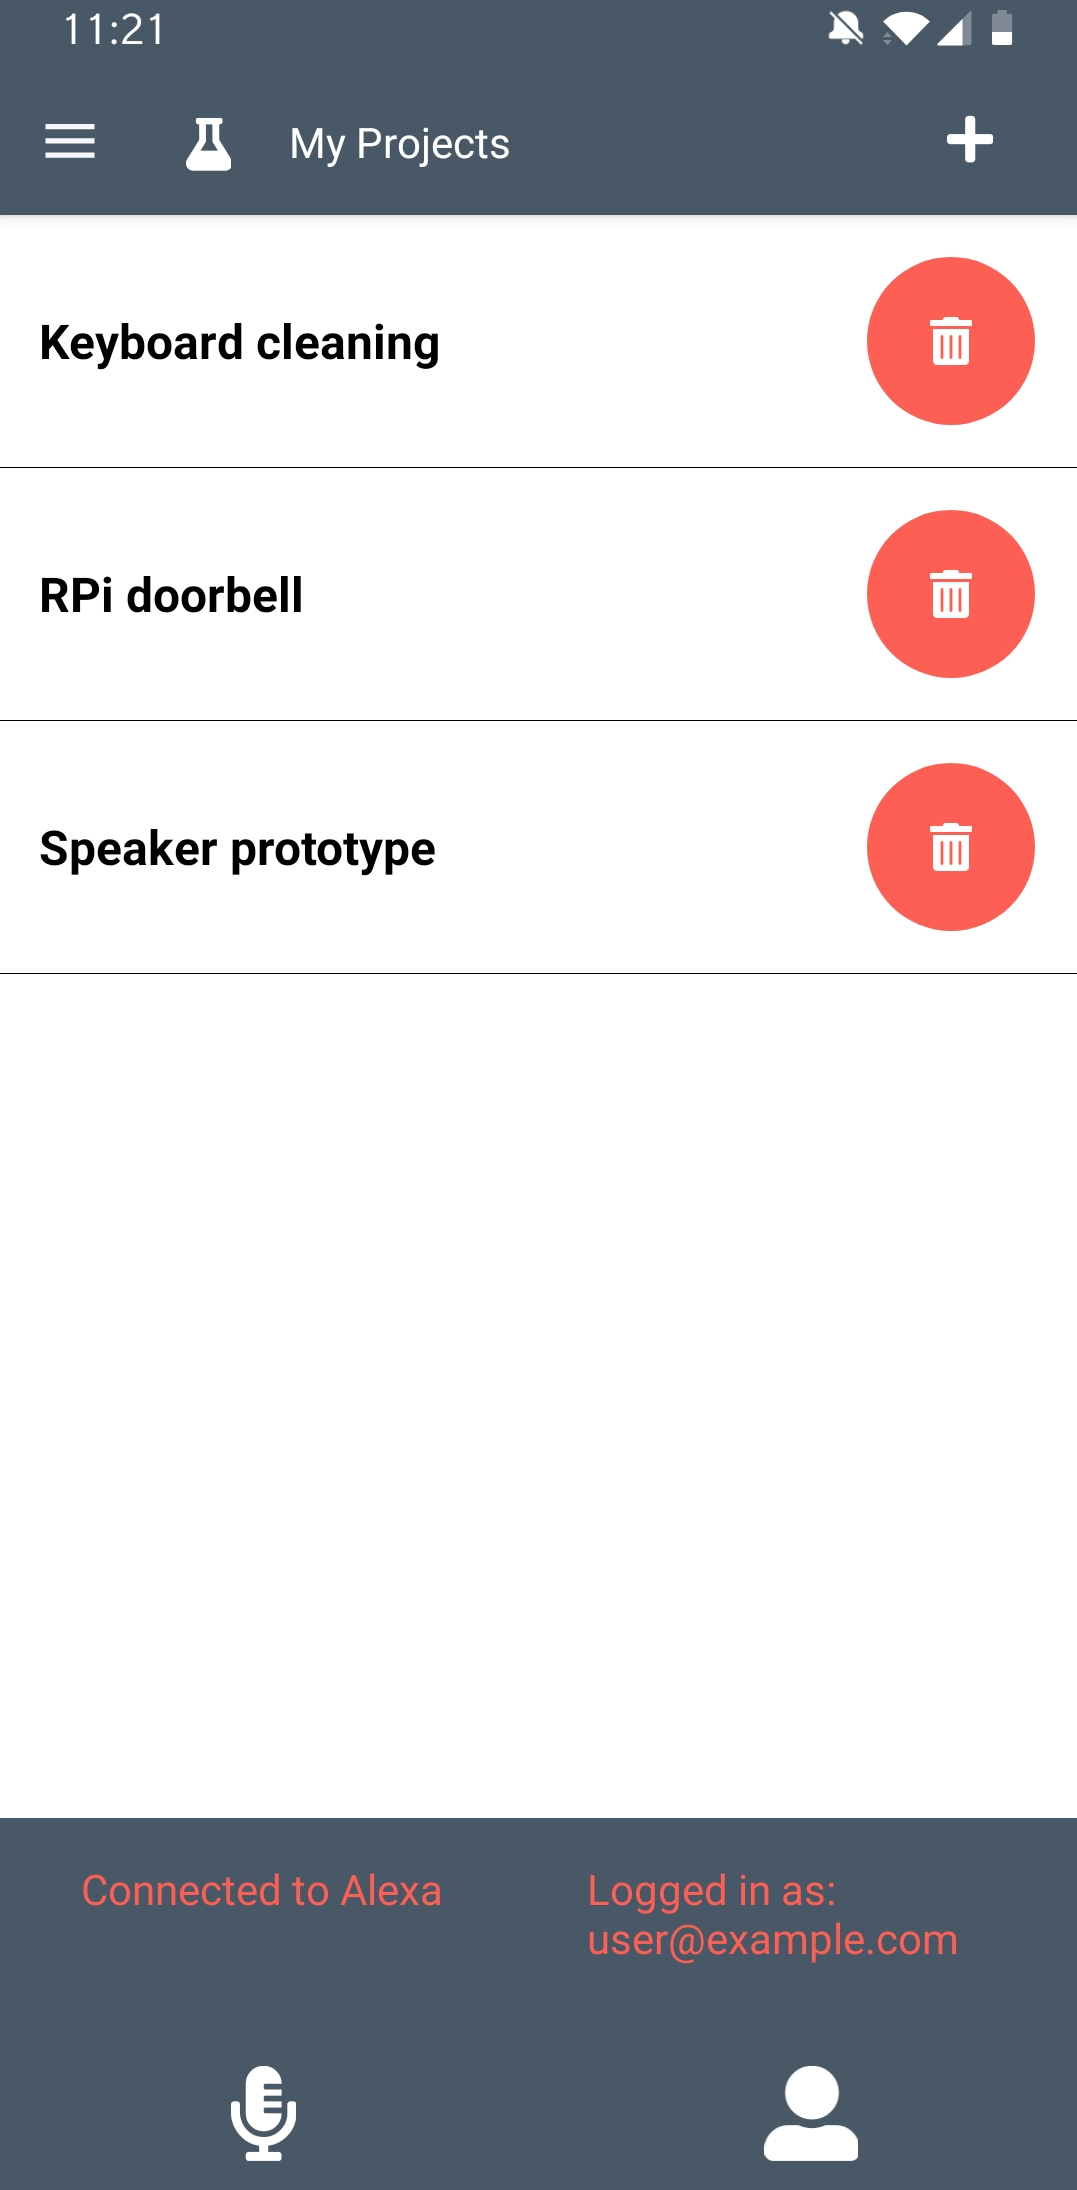
\includegraphics[width=5.5cm]{app_alexa_yes_small}
\end{center}
	\caption{Stran Dashboard v mobilni aplikaciji.}
\label{app_dashboard_first}
\end{figure}

% Pri dodajanju se v uporabnikovo zbirko doda nov prazen dnevnik z naslovom in opisom, ki ju vpiše uporabnik.
% Pri brisanju se morajo vsi podatki izbrisanega dnevnika odstraniti iz podatkovne baze.
% Ko uporabnik preko aplikacije odpre katerega od delavniških dnevnikov, mu strežnik vrne dnevnik in zbirko korakov, ki mu pripada.

% Avtenticiran uporabnik lahko dostopa do svoje zbirke delavniških dnevnikov.
% Vsak uporabnik lahko ima nič ali več delavniških dnevnikov.

% Če operacije nad delavniški API javi napako \texttt{Bad Request: Not Authorised}.

Uporabnik nov delavniški dnevnik ustvari tako, da pritisne na gumb z ikono + na strani Dashboard.
Odpre se obrazec za ustvarjanje projektov (na sliki \ref{app_create_new}), kamor vnese naslov, kratek opis projekta in opis možnih nevarnosti.
% DELJENJE
Te podatke ozadna koda aplikacije zapiše v objekt razreda \texttt{CreatePro-\\jectRequest}.

\begin{verbatim}
CreateProjectRequest { 
    string Title;  
    string Description; 
    string Dangers; 
} 
\end{verbatim}

\texttt{CreateProjectRequest} aplikacija pošlje na URL \enquote{\texttt{/projects/create}} preko metode POST.
Strežnik nato ustvari nov dnevnik s podatki iz prejete zahteve.
Odjemalcu se kot odgovor pošlje ustvarjen objekt tega projekta.

\begin{figure}[H]
\begin{center}
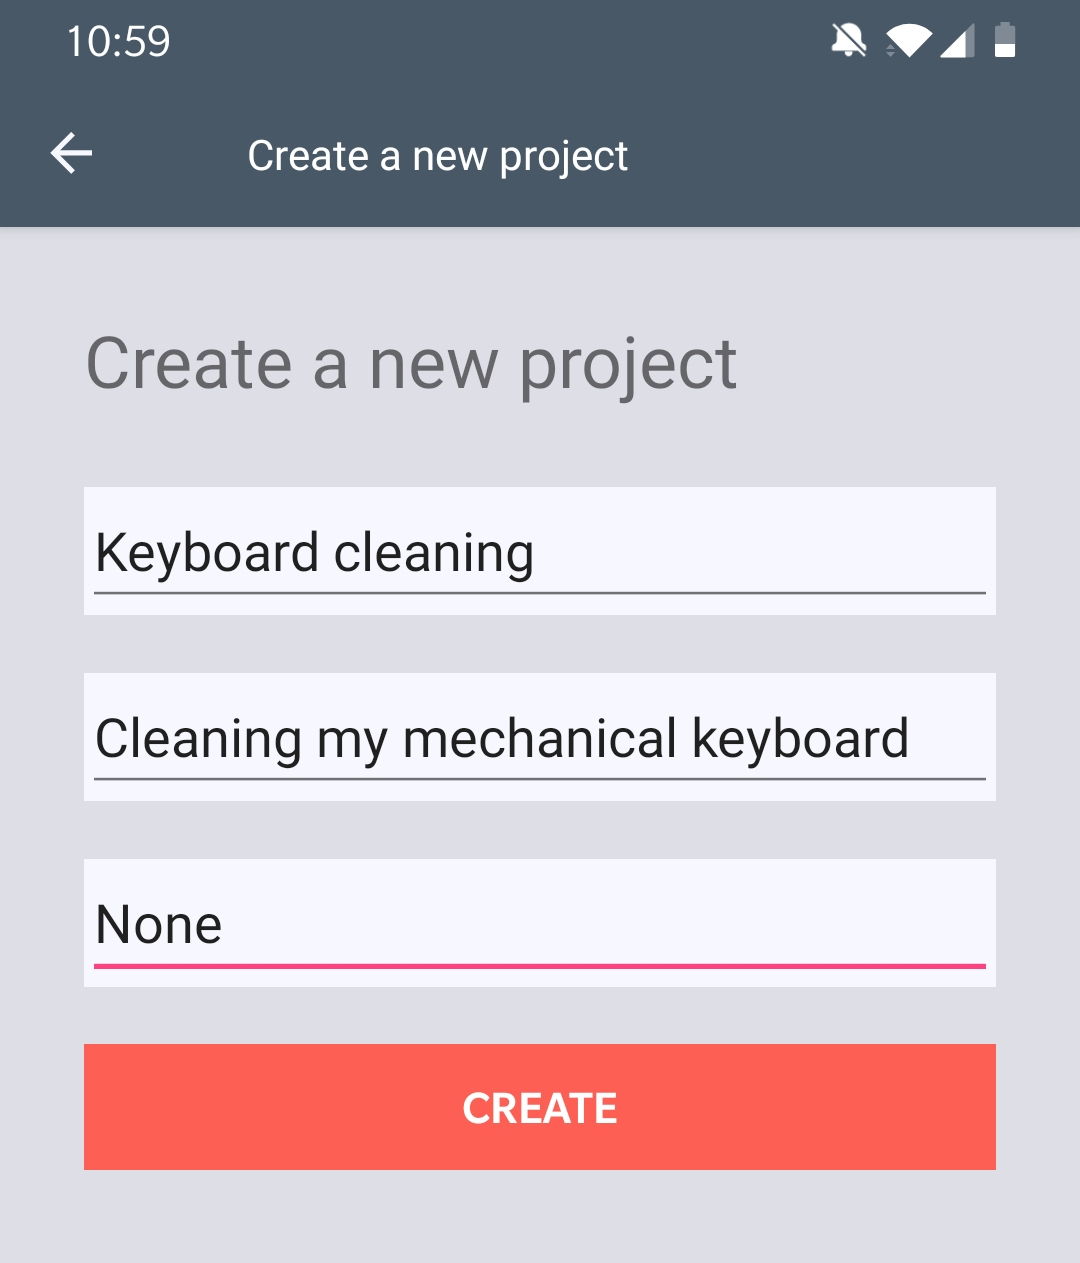
\includegraphics[width=6.5cm]{app_create_new_small}
\end{center}
	\caption{Obrazec za ustvarjanje novega projekta v aplikaciji.}
\label{app_create_new}
\end{figure}


\noindent Razred \texttt{Project} izgleda tako:

\begin{verbatim}
Project { 
    int Id; // unikatni identifikator 
    string Title; 
    string Description; 
    string Dangers; 
    IEnumerable<Note> Notes; // seznam korakov 
    ... 
}
\end{verbatim}

\begin{figure}[H]
\begin{center}
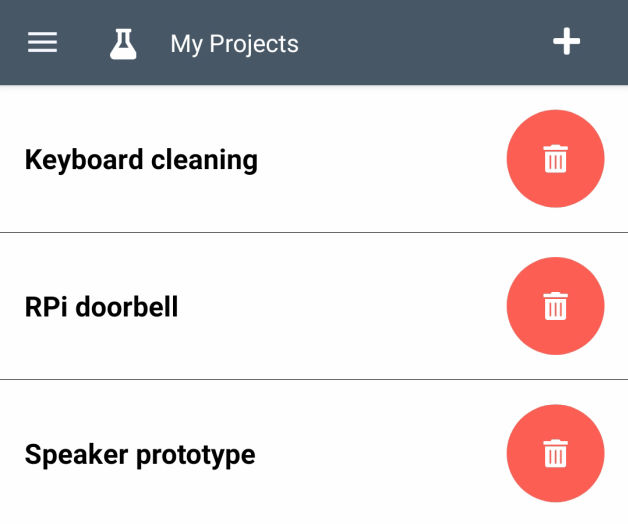
\includegraphics[width=6.5cm]{app_dashboard}
\end{center}
	\caption{Seznam delavniških dnevnikov v mobilni aplikaciji.}
\label{app_dashboard}
\end{figure}

Avtenticiran uporabnik lahko do svojih delavniških dnevnikov dostopa tako, da s seznama dnevnikov (na sliki \ref{app_dashboard}) izbere željenega.
Aplikacija pošlje avtoriziran GET zahtevek na URL \enquote{\texttt{/projects/\{id\}}}.
Polje \texttt{\{id\}} mora biti enolični identifikator projekta.
Strežnik uporabniku vrne kopijo objekta delavniškega dnevnika in pripadajočih korakov.


Uporabnik lahko delavniški dnevnik izbriše tako, da pritisne na gumb z ikono smetnjaka (na sliki \ref{app_dashboard}) ob naslovu odvečnega dnevnika.
Aplikacija pošlje DELETE zahtevo na URL \enquote{\texttt{/projects/\{id\}}}.
Če zahteva ni avtorizirana z ustreznim žetonom, se projekt ne izbriše.



\subsection{Operacije s koraki delavniškega dnevnika}

Korak delavniškega dnevnika opisuje eno od nalog v tehnološkem postopku.

Delavniški dnevnik lahko vsebuje tudi slikovno gradivo.
Korake smo ločili na slikovne in besedilne.
Besedilni korak vsebuje naslov, besedilo in trajanje naloge, ki jo opisuje, slikovni pa vsebuje tudi fotografijo.

Sistem podpira dodajanje in brisanje korakov, spreminjanje vsebine posameznega koraka in spreminjanje vrstnega reda korakov.


\subsubsection{Dodajanje besedilnega koraka}

Uporabnik v odprt projekt besedilni korak vstavi s pritiskom na gumb s črko T (na sliki \ref{app_project_note} levo).
Odpre se obrazec za dodajanje koraka (na sliki \ref{app_project_note} na sredini).
Obrazec ima polja za naslov, besedilo in trajanje.

\begin{figure}[H]
\begin{center}
	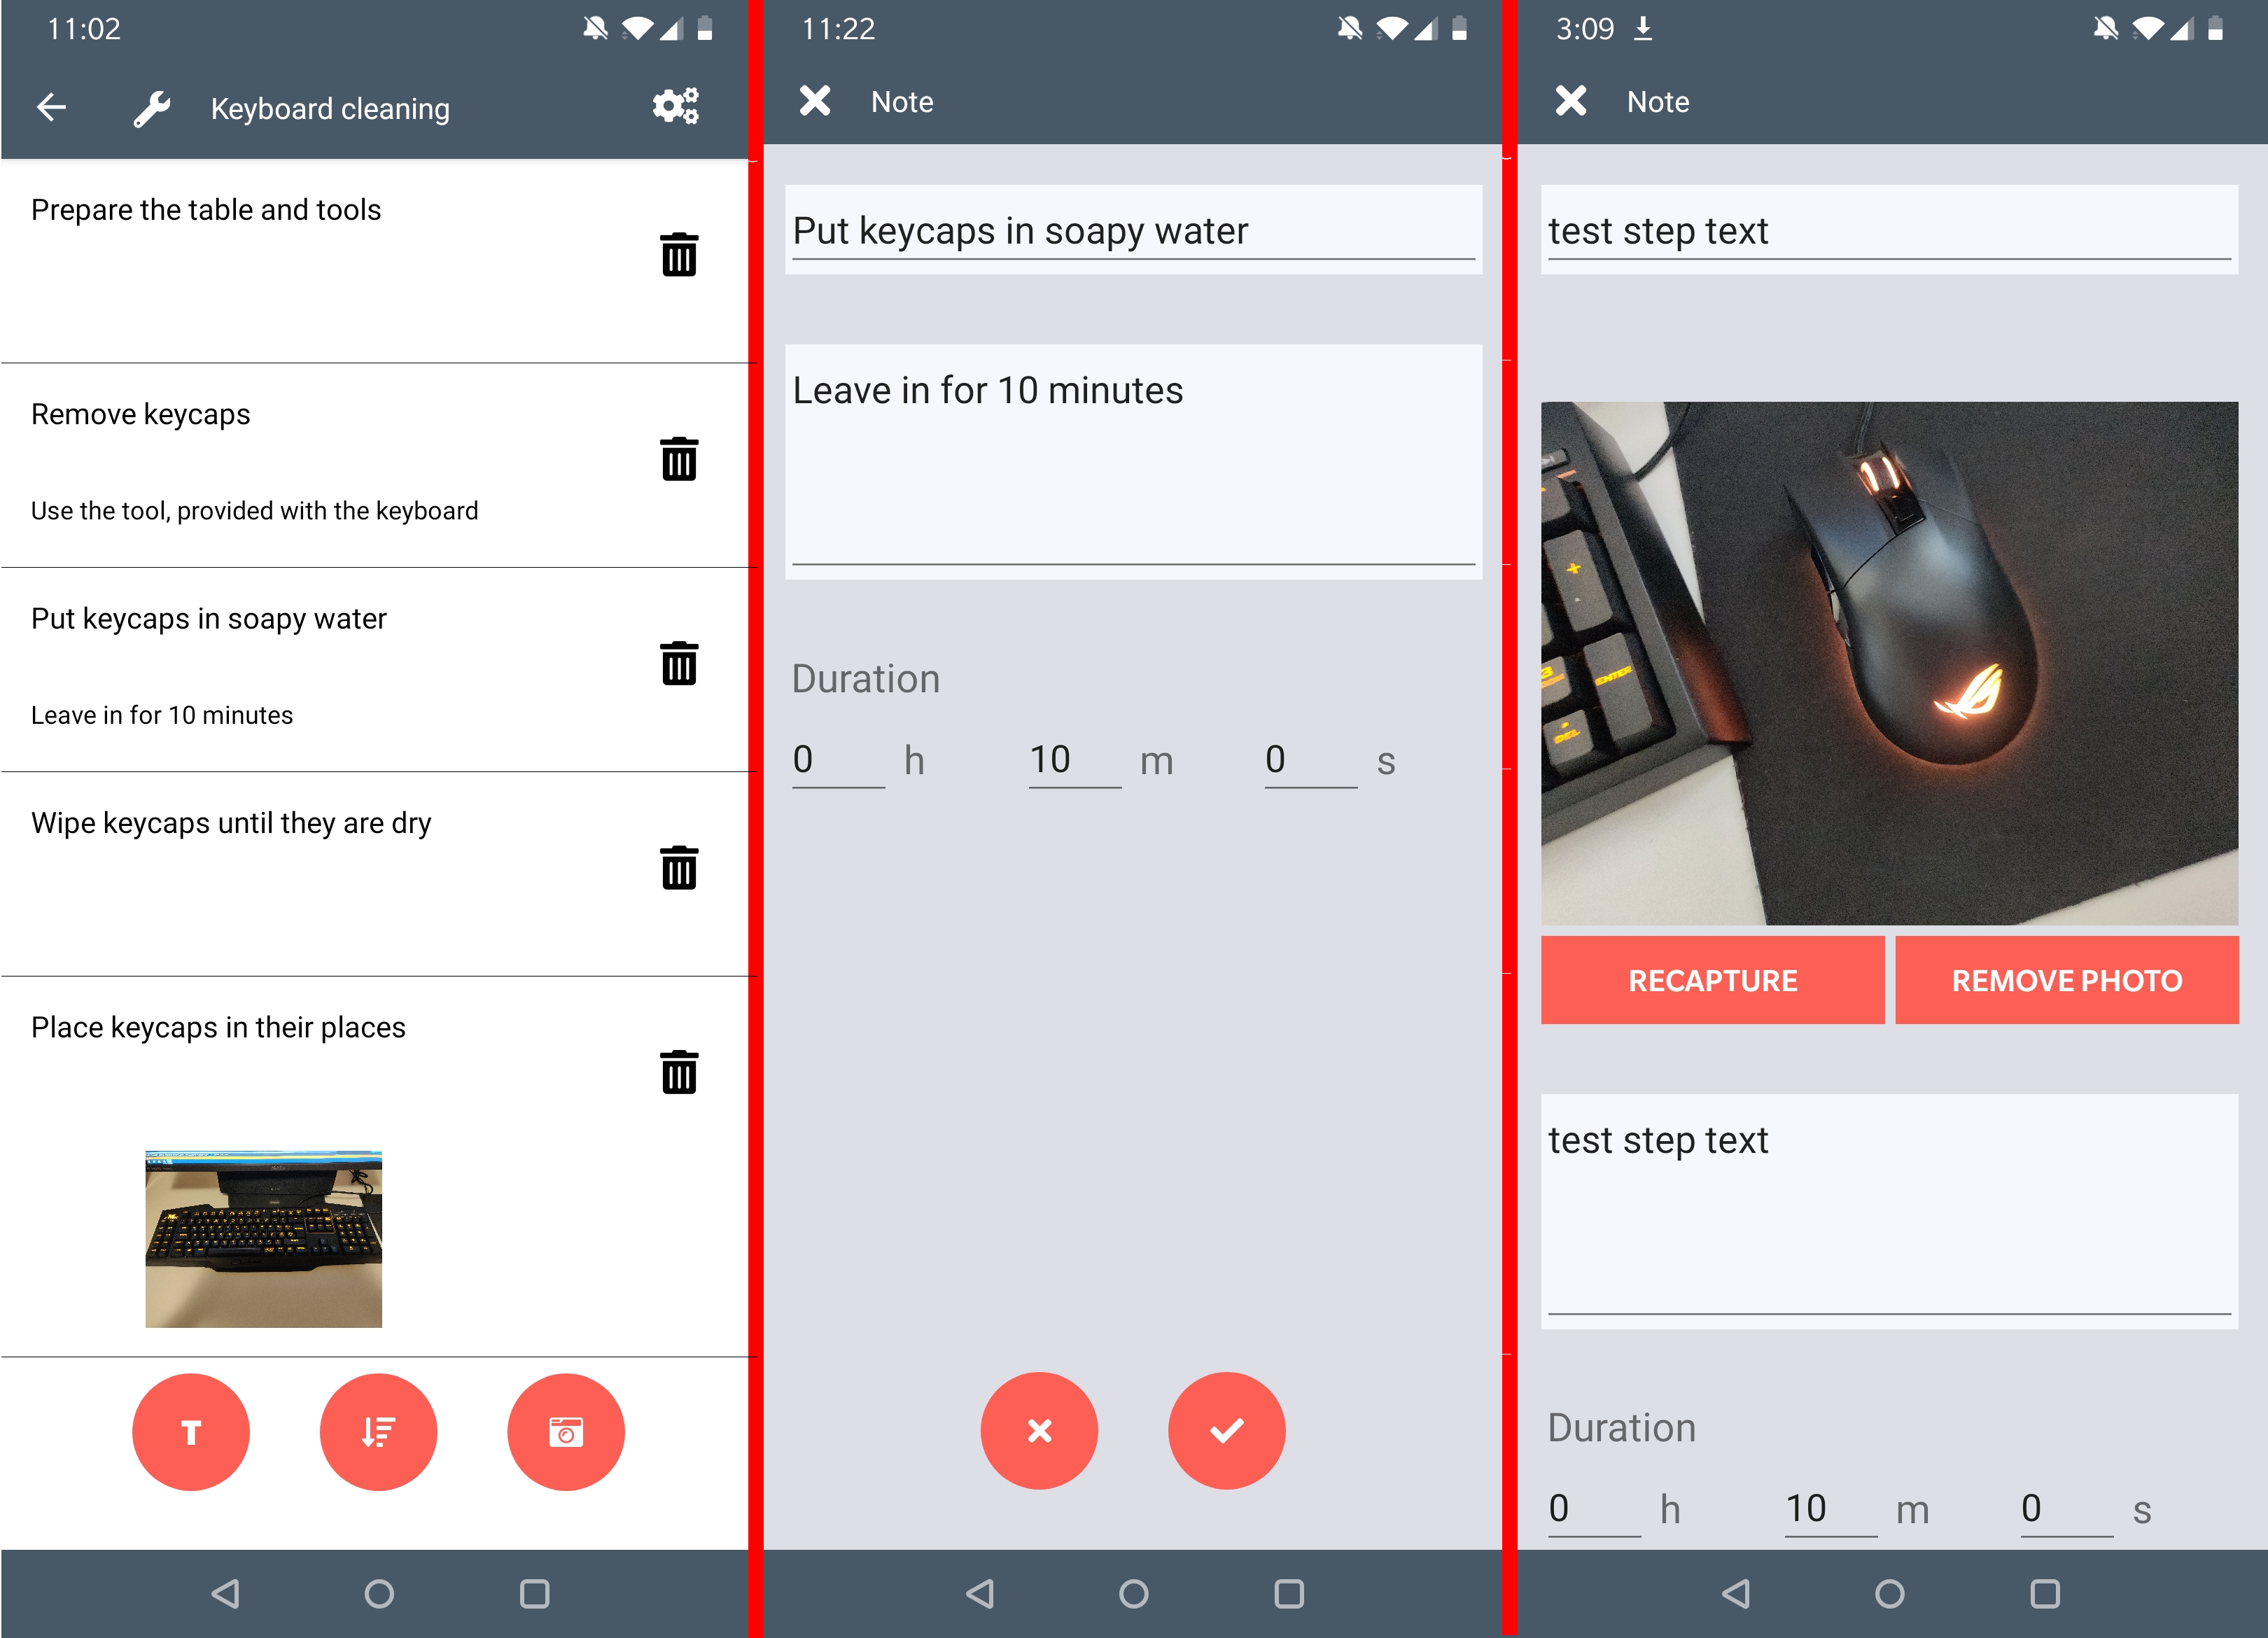
\includegraphics[width=13.5cm]{app_project_note}
\end{center}
	\caption{Stran za pregled delavniškega dnevnika in obrazci za dodajanje besedilnih in slikovnih korakov v mobilni aplikaciji.}
\label{app_project_note}
\end{figure}

Vsebino teh polj ozadna koda aplikacije zapiše v objekt razreda \texttt{Note}.
Naslov koraka se zapiše v polje Title, opis v polje Text, trajanje pa se zapiše v polja Hours, Minutes in Seconds.
\begin{verbatim}
Note { 
    ... 
    string Title; 
    string Text; 
    int Hours; 
    int Minutes;
    int Seconds;
    ...
}
\end{verbatim}

% DELJENJE
Ustvarjen objekt razreda \texttt{Note} aplikacija pošlje na URL \enquote{\texttt{/projects/\{id\}-\\/addnote}} preko metode POST.
Polje \texttt{\{id\}} mora biti enolični identifikator projekta, ki mu želimo dodati korak.

Strežnik prejet korak vstavi v projekt.
Aplikaciji v odgovor vrne kopijo ustvarjenega koraka na strežniku, ki ga aplikacija doda zbirki korakov trenutno odprtega projekta.



\subsubsection{Dodajanje slikovnega koraka}

Za hranjenje besedilnih in slikovnih korakov smo zaradi preprostosti implementacije uporabili isti razred (\texttt{Note}).
Besedilni in slikovni korak se ločita v vrednosti boolean zastavice \texttt{IsImage}.
Besedilni korak ima to polje nastavljeno na vrednost \texttt{false}, slikovni pa na \texttt{true}.

\begin{Verbatim}[commandchars=+\[\]]
Note { 
    +underline[bool IsImage;]
    string Title; 
    string Text; 
    int Hours; 
    int Minutes;
    int Seconds; 
    +underline[string Url;] // Lokacija slike na odjemalcu 
    +underline[string ServerUrl;] // Lokacija slike na strežniku
    ... 
}
\end{Verbatim}

Uporabnik slikovni korak vstavi v projekt s pritiskom na gumb z ikono kamere (na sliki \ref{app_project_note} levo).

Odpre se privzeta aplikacija za kamero, s katero uporabnik zajame fotografijo.
Po zajemu se odpre obrazec za dodajanje koraka (na sliki \ref{app_project_note} desno).
Fotografija se zašifrira v znakovni niz po metodi Base64.
Vsebina vnosnih polj obrazca za naslov, besedilo in trajanje koraka se zapiše v objekt razreda \texttt{Note}.

Korak in šifrirana fotografija se zapišeta v zahtevek \texttt{UploadImageRequest}.

\begin{verbatim}
UploadImageRequest { 
    Note Note; 
    string ImageString; 
}
\end{verbatim}

Polje \texttt{ImageString} vsebuje v znakovni niz šifrirano fotografijo.
Polje \texttt{Note} vsebuje korak delavniškega dnevnika.
Ta objekt aplikacija pošlje preko POST metode na URL \enquote{\texttt{/projects/\{id\}/addimage}} (slika \ref{app_code_image}).

\begin{figure}[H]
\begin{center}
	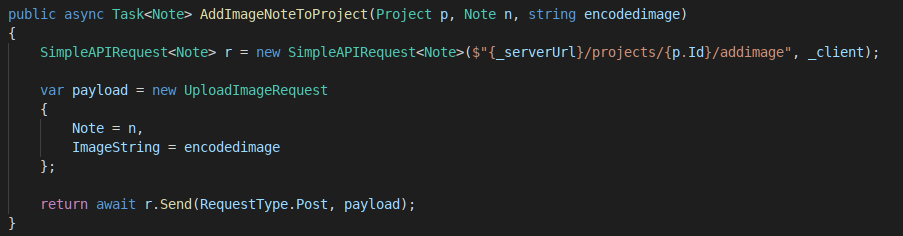
\includegraphics[width=13.5cm]{app_code_image}
\end{center}
	\caption{Koda za ustvarjanje in pošiljanje zahtevka za dodajanje slikovnega koraka v aplikaciji.}
\label{app_code_image}
\end{figure}


Strežnik prejet korak vstavi v projekt in dešifrira sliko iz znakovnega niza nazaj v slikovno datoteko.
Slikovno datoteko nato hrani v svojem datotečnem sistemu.
Lokacija fotografije v datotečnem sistemu strežnika se zapiše v polje \texttt{ServerUrl}.

Aplikaciji v odgovor vrne kopijo ustvarjenega koraka na strežniku, ki ga aplikacija doda zbirki korakov trenutno odprtega projekta.


% Poljema \texttt{Url} in \texttt{ServerUrl} se dodeli vrednost samo pri slikovnih korakih.
% Polje \texttt{Url} hrani lokacijo fotografije na odjemalcu, \texttt{ServerUrl} pa lokacijo fotografije na strežniku.
% Ko se na odjemalcu zajame fotografija, odjemalec nastavi vrednost polja \texttt{Url} na lokacijo ustvarjene fotografije v datotečnem sistemu.
% 
% Polje \texttt{ServerUrl} se nastavi na strežniku.
% Strežnik vstavi prejet korak iz zahteve \texttt{UploadImageRequest} in ga zapiše v podatkovno bazo.
% \texttt{ImageString} se dekodira v slikovno datoteko in hrani na strežniku.
% Ko se fotografija uspešno zapiše v datotečni sistem, se v polje \texttt{ServerUrl} v pripadajočem koraku zapiše lokacija fotografije na strežniku.
% 



\subsubsection{Urejanje korakov v projektu}

Uporabnik lahko korake v delavniških dnevnikih posodablja.
Spreminja lahko njihovo vsebino, naslov in trajanje.
Obrazec za urejanje koraka odpre tako, da v seznamu korakov projekta (na sliki \ref{app_project_note} levo) pritisne na besedilo koraka, ki ga želi posodobiti. 

% DELJENJE
Uporabnik korak posodobi s PUT zahtevo na URL \enquote{\texttt{/projects/\{pid\}/-\\update/\{nid\}}}.
Polje \{pid\} je enolični identifikator projekta, ki si lasti korak, \{nid\} pa enolični identifikator koraka, ki ga želimo posodobiti.
Telo zahteve mora vsebovati objekt razreda \texttt{Note}, ki ga je uporabnik posodobil.

% DELJENJE
Uporabnik slikovni korak posodobi s PUT zahtevo na naslov \enquote{\texttt{/projects-\\/\{pid\}/update/\{nid\}/image}}.
Polje \{pid\} je enolični identifikator projekta, ki si lasti korak, \{nid\} pa enolični identifikator koraka, ki ga želimo posodobiti.
Telo te zahteve mora vsebovati zahtevek \texttt{UploadImageRequest}.
V \texttt{UploadImageRequest} mora biti polje \texttt{Note} objekt, ki ga želimo posodobiti.
Polje \texttt{ImageString} mora biti šifrirana slika, ki bo zamenjala prejšnjo sliko.
Slika mora biti šifrirana po metodi Base64.



\subsubsection{Brisanje korakov v projektu}

Korak lahko uporabnik iz projekta izbriše tako, da pritisne gumb z ikono črnega smetnjaka ob koraku (na sliki \ref{app_project_note} levo).

% DELJENJE
Ozadna koda aplikacije pošlje DELETE zahtevo na URL \enquote{\texttt{/projects/-\\\{pid\}/delete/\{nid\}}}.
Polje je \texttt{\{pid\}} enolični identifikator projekta, v katerem se nahaja korak, \texttt{\{nid\}} pa enolični identifikator koraka, ki ga želimo izbrisati.

Če ima korak nastavljeno polje \texttt{IsImage} na \texttt{true}, se poleg zapisa v bazi izbriše tudi pripadajoča slikovna datoteka.



\subsubsection{Spreminjanje vrstnega reda korakov v projektu}

% Sistem mora podpirati tudi 
Uporabnik lahko korakom v svojih projektih spreminja vrstni red prikaza.
Na strani za urejanje dnevnika pritisne gumb z ikono seznama (na sliki \ref{app_ordering} levo).
To na strani za urejanje dnevnika zažene način za spreminjanje vrstnega reda korakov (na sliki \ref{app_ordering} v sredini).
Uporabnik v tem načinu pritisne na korak, ki ga želi prestaviti.
Izbran korak se obarva oranžno.
Izbran korak premakne navzgor ali navzdol po seznamu z gumbi z ikono puščic (na sliki \ref{app_ordering} desno).
Nazaj v način za dodajanje se uporabnik vrne s pritiskom na gumb z ikono nalivnika.

\begin{figure}[H]
\begin{center}
	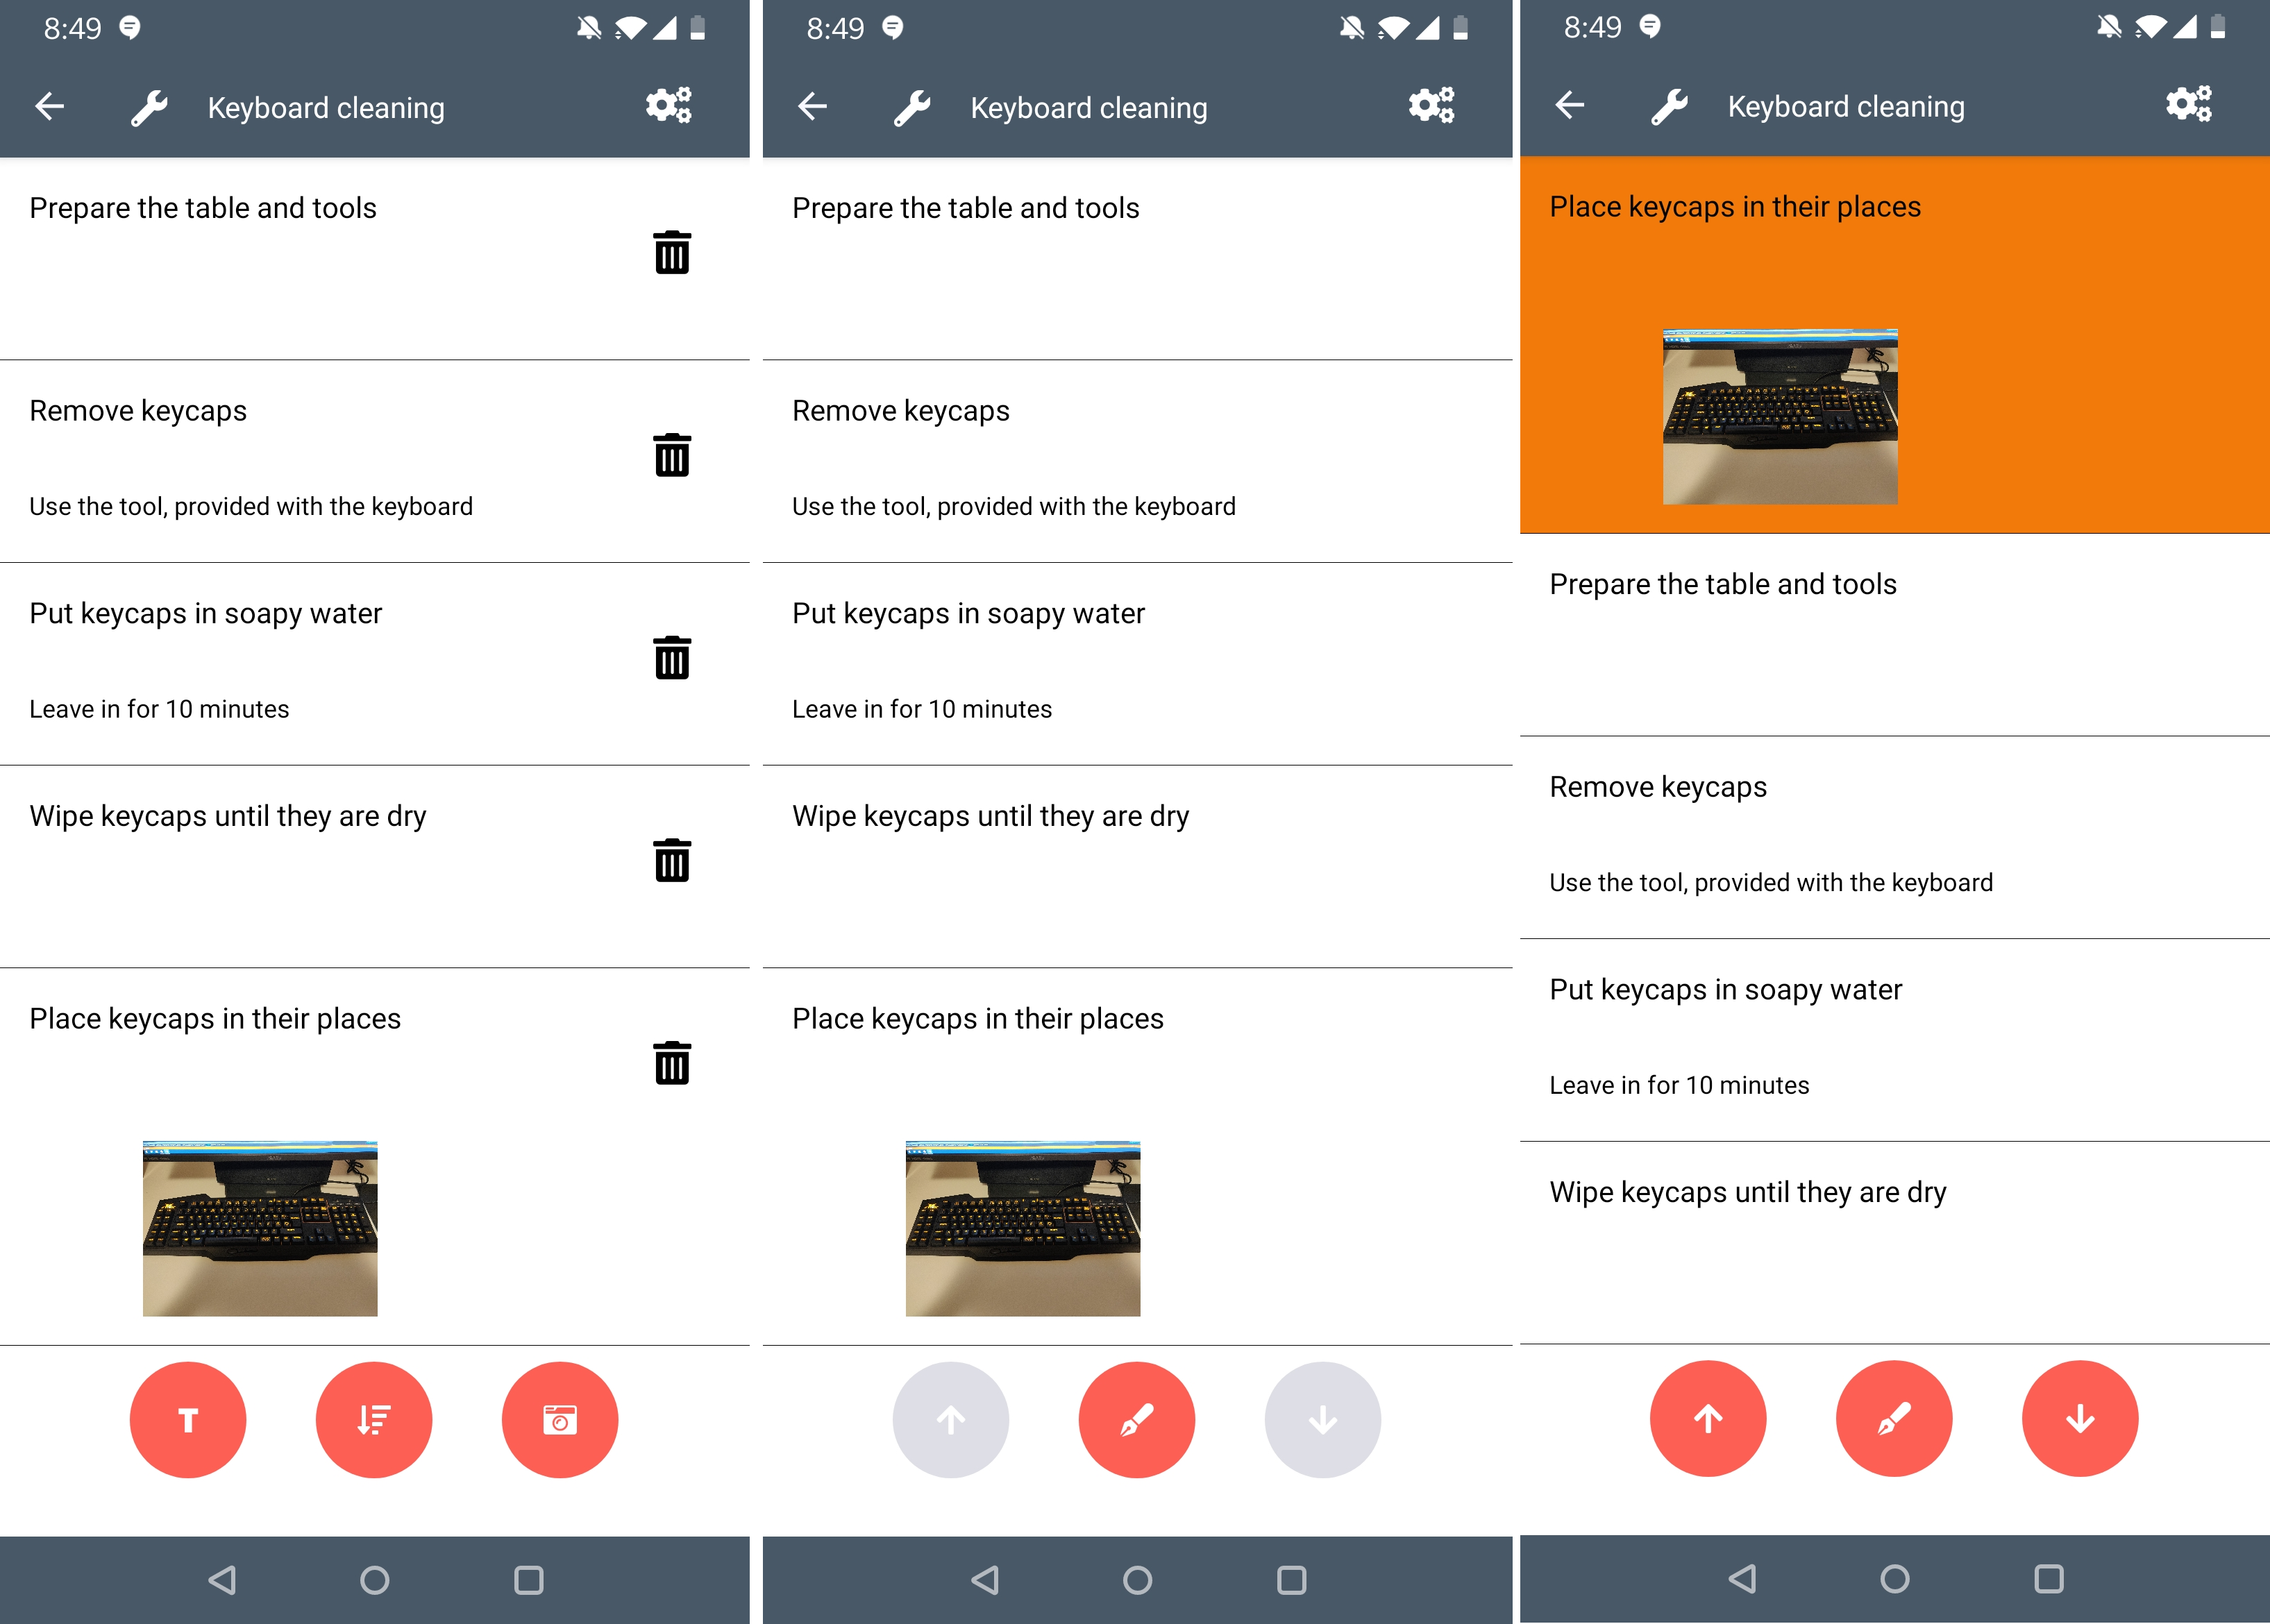
\includegraphics[width=13.5cm]{app_ordering}
\end{center}
	\caption{Koda za ustvarjanje in pošiljanje zahtevka za dodajanje slikovnega koraka v aplikaciji.}
\label{app_ordering}
\end{figure}

Položaj koraka \texttt{Note} v projektu lahko razberemo iz atributa \texttt{Position}.
Prvi korak ima \texttt{Position} 0, drugi 1, tretji 2 itd.


\begin{Verbatim}[commandchars=+\[\]]
Note { 
    int Id; 
    +underline[int Position;]
    bool IsImage;  
    string Title; 
    string Text;
    int Hours; 
    int Minutes;
    int Seconds;
    string Url;
    string ServerUrl;
}
\end{Verbatim}

% Pri dodajanju korakov v projekt se obstoječe korake projekta razvrsti po vrednosti polja \texttt{Position}.
% Najdemo največjo vrednost tega polja, ki se v seznamu pojavi in ji prištejemo 1.
% Nato to vrednost priredimo polju \texttt{Position} novo kreiranega koraka.

Ob spremembi pozicije koraka v projektu, ozadna koda aplikacije pošlje zahtevo PUT na URL \enquote{\texttt{/projects/\{pid\}/\{nid\}/\{positions\}}}.

Polje \texttt{\{pid\}} je enolični identifikator projekta, v katerem se nahaja korak.
Polje \texttt{\{nid\}} je enolični identifikator koraka \texttt{Note}.
Polje \texttt{\{positions\}} vsebuje število, ki pove, za koliko mest želimo korak prestaviti.
To število je lahko pozitivno ali negativno celo število.
Negativna vrednost \texttt{\{positions\}} prestavi korak proti začetku seznama, pozitivna pa proti koncu.

Implementacijo spreminjanja vrstnega reda korakov na strežniku prikazuje spodnja slika (\ref{api_code_changepos}).

\clearpage

\begin{figure}[H]
\begin{center}
	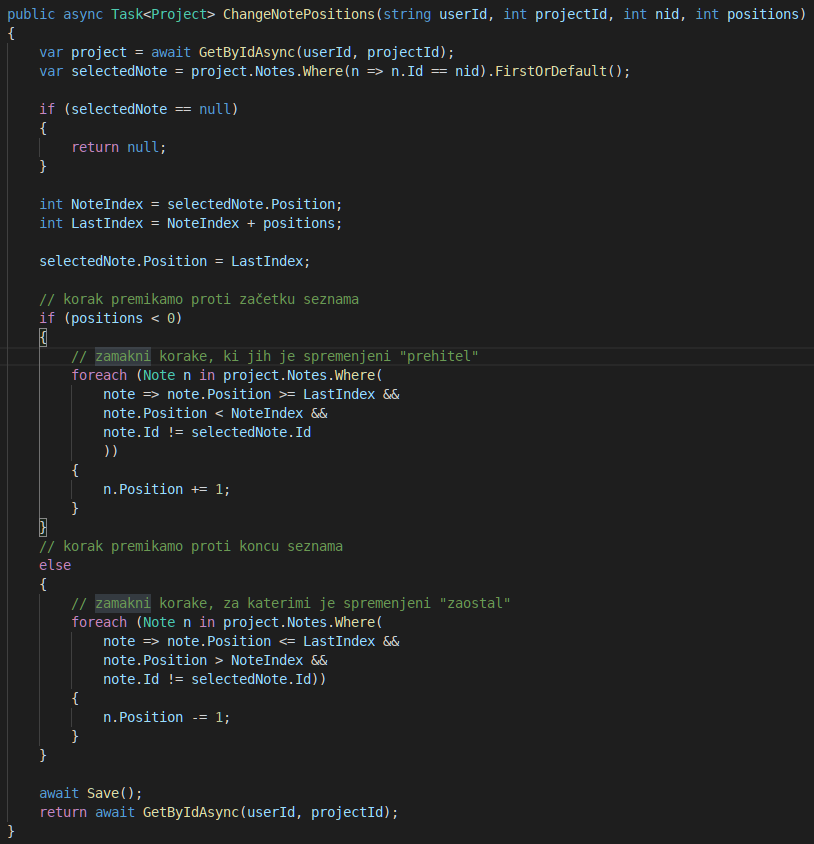
\includegraphics[width=13.5cm]{api_code_changepos}
\end{center}
	\caption{Koda za spreminjanje vrstnega reda korakov delavniškega dnevnika na strežniku.}
\label{api_code_changepos}
\end{figure}



\subsection{Izvoz projektov}

Sistem omogoča izvoz delavniških dnevnikov v druge računalniške formate.
Izvoženi delavniški dnevniki lahko služijo kot varnostna kopija.
Izvozimo jih lahko v besedilno datoteko ali HTML dokument (slika \ref{app_project_export}).

\begin{figure}[H]
\begin{center}
	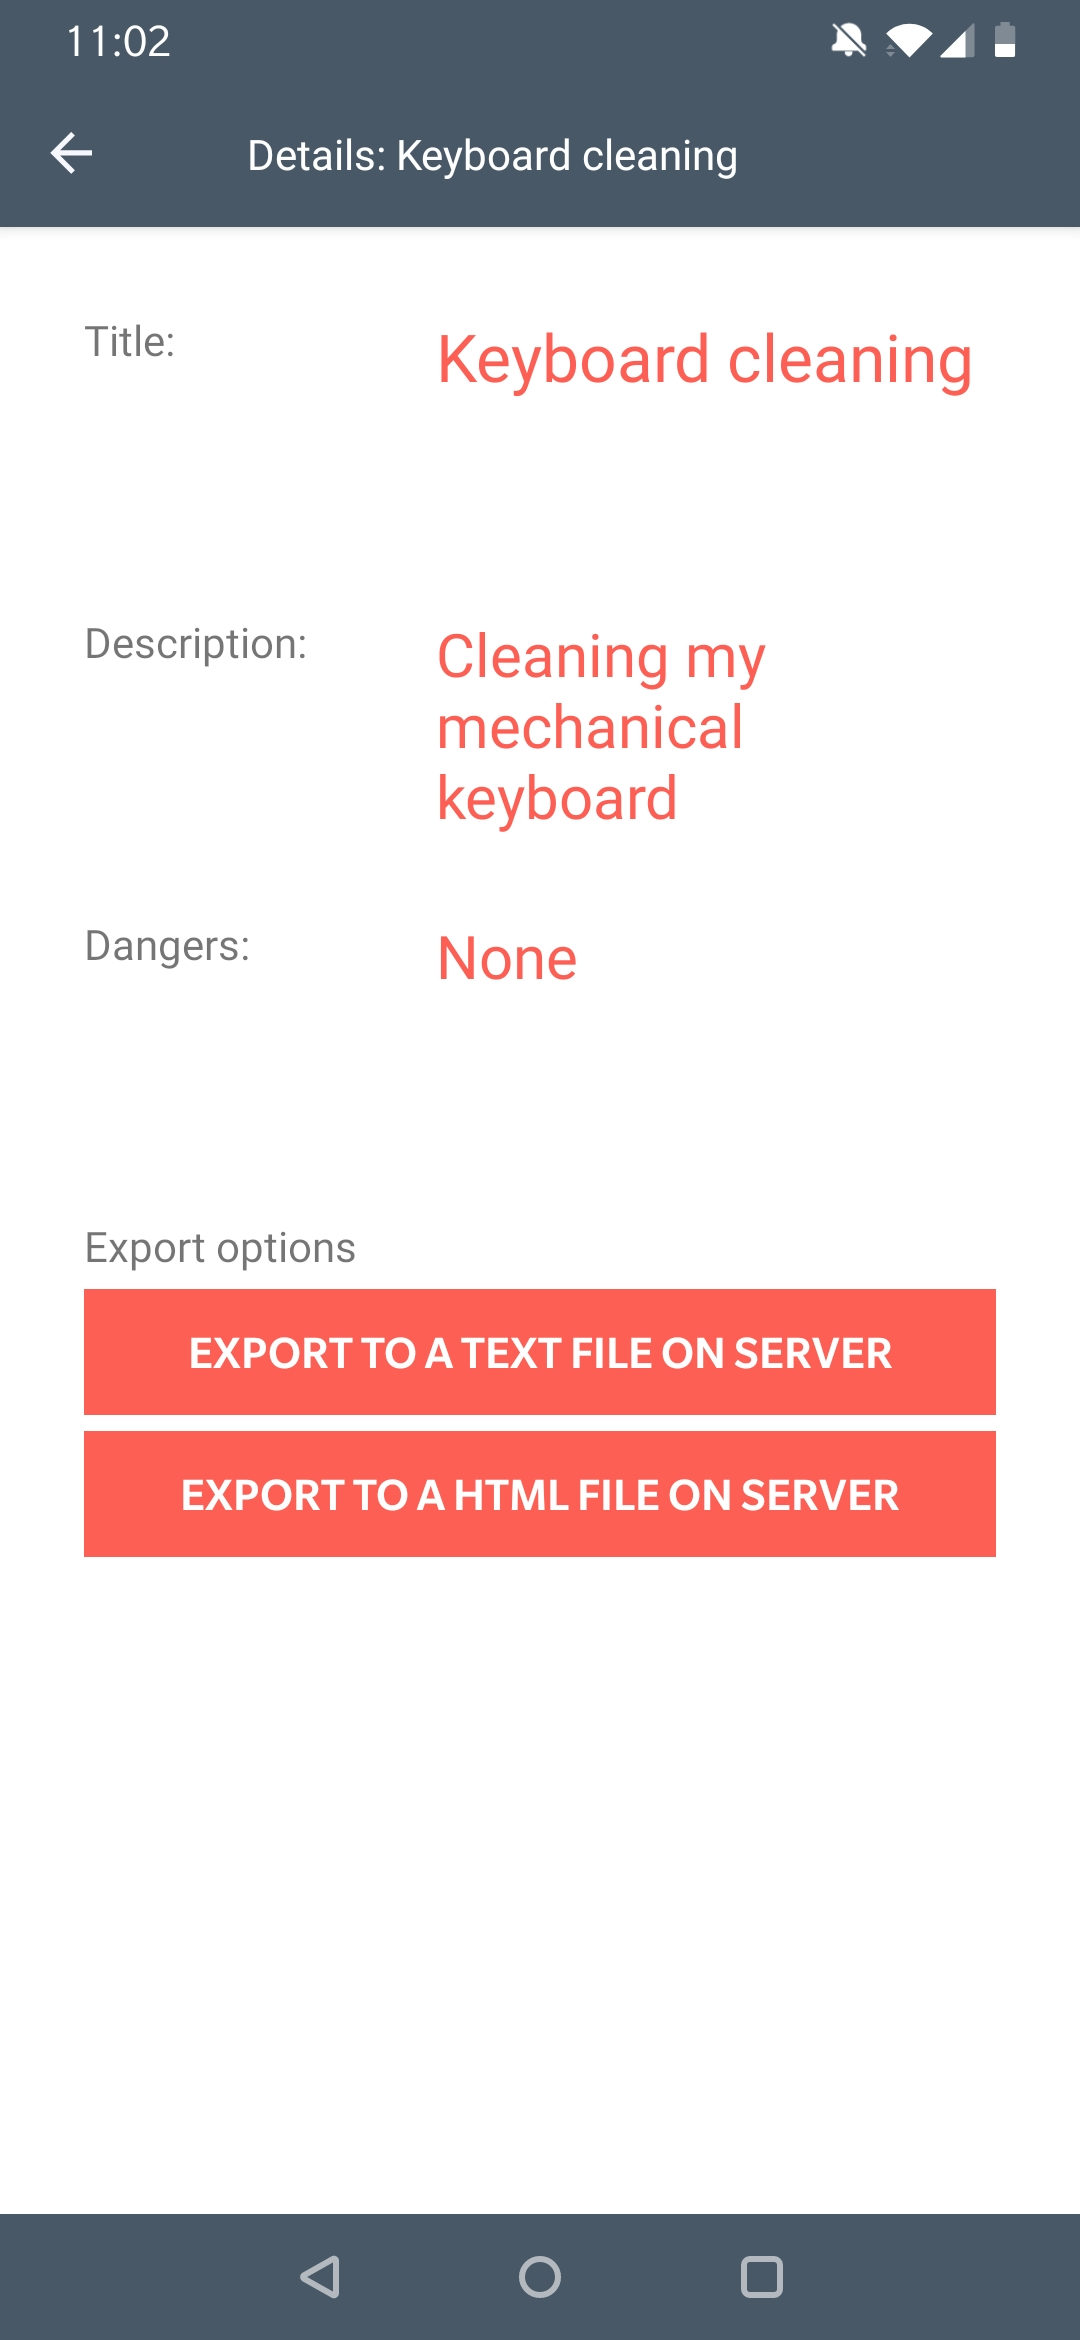
\includegraphics[width=6cm]{app_project_export}
\end{center}
	\caption{Stran za izvoz projektov v mobilni aplikaciji.}
\label{app_project_export}
\end{figure}

Uporabnik projekt izvozi tako, da odpre stran s podrobnostmi dnevnika.
To stran odpre s klikom na gumb z ikono zobnika na vrhu strani za prikaz projekta.
Na strani s podrobnostmi dnevnika ima dva oranžna gumba (slika \ref{app_project_export}).
S pritiskom na zgornji gumb izvozi projekt v besedilno datoteko, s pritiskom na spodnji gumb pa v HTML dokument.

V besedilno datoteko se projekt izvozi tako, da aplikacija pošlje GET zahtevo na URL \enquote{\texttt{/projects/\{id\}/export/text}}.
Strežnik v besedilno datoteko vpiše naslov, opis projekta in možne nevarnosti pri delu.
Nato korake uredi naraščajoče po vrednosti stolpca \texttt{Position} in jih enega za drugim zapiše v datoteko.
Pri slikovnih korakih se zapiše besedilo in lokacija pripadajoče fotografije.

V HTML dokument se dnevnik izvozi tako, da aplikacija pošlje GET zahtevo na URL \enquote{\texttt{/projects/\{id\}/export/html}}.
Pri izvozu v HTML dokument (slika \ref{export_html}) se naslov projekta zapiše kot HTML naslov H1, opis projekta kot naslov H2, koraki pa kot HTML odstavki.
V HTML dokumentu lahko prikažemo poleg besedila slikovnih korakov tudi slike.

\begin{figure}[H]
\begin{center}
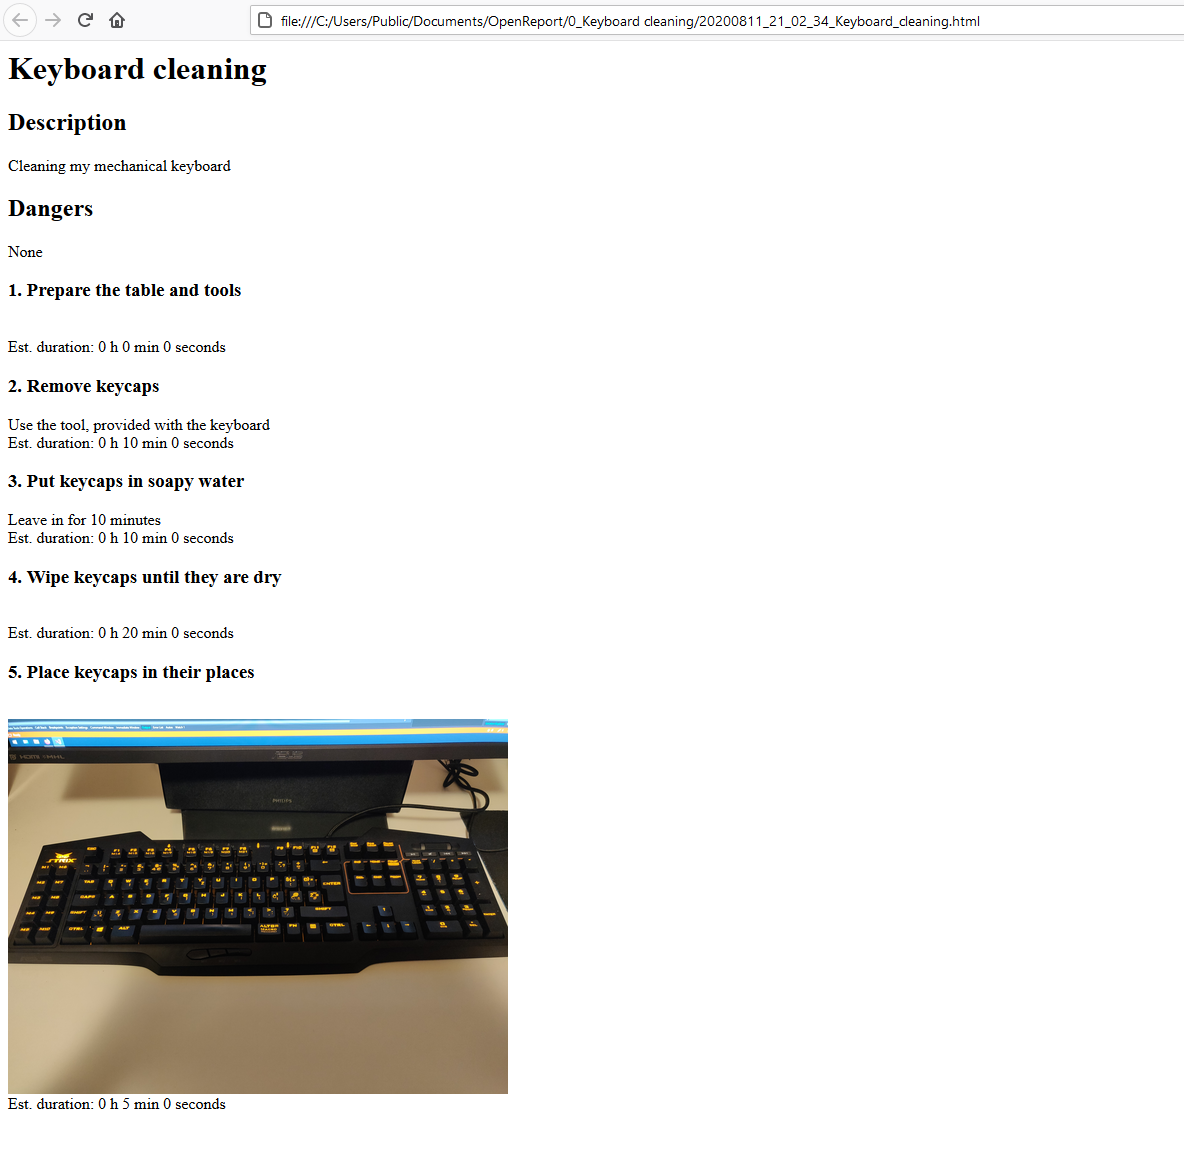
\includegraphics[width=13cm]{export_html}
\end{center}
\caption{Projekt, izvožen v HTML dokument.}
\label{export_html}
\end{figure}

Lokacija izvožene datoteke se nahaja v polju \texttt{FolderLocation} v razredu \texttt{Project}.
Privzeta lokacija, ki se nastavi ob ustvarjanju projekta je 
\\\enquote{\texttt{C:/users/\$USER/Public Documents/OpenReport}}.

\begin{Verbatim}[commandchars=+\[\]]
Project {
    int Id; 
    string Title; 
    string Description; 
    string Dangers; 
    +underline[string FolderLocation;] // lokacija pripadajočih datotek 
    IEnumerable<Note> Notes; 
    ... 
}
\end{Verbatim}






\subsection{Uporaba kamere v Xamarin}

Za uporabo kamere v ogrodju Xamarin smo uporabili vtičnik Xam.Plugin.Media \cite{xampluginmedia}.
Vtičnik je licensiran pod MIT licenco.

Zanj smo se odločili, ker podpira zajem fotografij s privzeto aplikacijo za zajemanje fotografij.
Izbiramo lahko tudi kvaliteto zajete fotografije.

Pred zajemom slike najprej preverimo, ali ima aplikacija na mobilni napravi zadostna dovoljenja.
Imeti mora dovoljenje za dostop do shrambe, fotografij in kamere.

Fotografijo zajamememo z metodo \texttt{TakePictureAsync}.
Zajeto fotografijo aplikacija hrani v objektu razreda ImageSource.
Fotografijo v tej obliki se lahko prikaže v XAML z grafičnim elementom Image.
Lahko jo zakodiramo v znakovni niz in pošljemo na strežnik.




\section{Uvedba glasovnega pomočnika}

Po implementaciji strežnika in mobilne aplikacije smo se lotili uvajanja glasovnega pomočnika v sistem OpenReport.

\subsection{Funkcionalne zahteve Alexa veščine}

Alexina veščina je program, ki glasovnemu pomočniku Amazon Alexa doda funkcionalnosti.
Alexo in zasnovano veščino smo uporabili kot dodaten uporabniški vmesnik za upravljanje z mobilno aplikacijo.

\noindent Z njim smo želeli doseči:
\begin{itemize}
	\item prostoročno narekovnaje besedilnega koraka,
	\item prostoročno odpiranje obrazca za dodajanje korakov v odprt projekt in
	\item prostoročno odpiranje kamere in dodajanje slikovnega koraka v projekt.
\end{itemize}


\subsection{Komunikacija strežnika z Amazon Alexo}

\begin{figure}[H]
\begin{center}
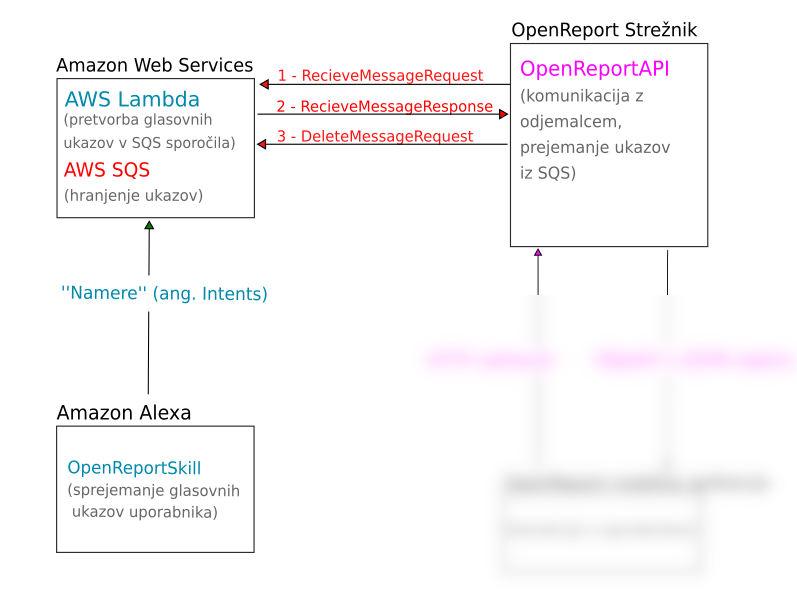
\includegraphics[width=13cm]{plan_sqs_server_alexa}
\end{center}
\caption{Komunikacija med strežnikom in glasovnim pomočnikom preko SQS.}
\label{plan_sqs_server_alexa}
\end{figure}


Strežnik z glasovnim pomočnikom Amazon Alexa komunicira (slika \ref{plan_sqs_server_alexa}) preko storitve Simple Queue Service (SQS). % iz sklopa storitev Amazon Web Services.
Amazon Alexa rezultate obdelanih glasovnih ukazov odloži v SQS vrsto, strežnik pa jih iz te vrste prebere.

SQS vrsta FIFO je sklad besedilnih sporočil.
Nanjo lahko pošiljamo nova sporočila ter beremo in brišemo obstoječa sporočila.

Glasovni pomočnik od uporabnika prejme izgovorjen glasovni ukaz.
Na podlagi tega ukaza glasovni pomočnik na SQS vrsto odloži tri različna besedilna sporočila:
% Strežnik periodično prejema sporočila iz SQS vrste.
% Ko sporočilo prejme, na podlgi njegove vsebine izvede eno od treh možnih funkcij.
\begin{itemize}
	\item Sporočilo \textbf{\enquote{addnote}} sporoči strežniku, naj na odjemalcu odpre obrazec za dodajanje besedilnega koraka.
	\item Sporočilo  \textbf{\enquote{addimage}} sporoči strežniku, naj na odjemalcu odpre kamero za dodajanje slikovnega koraka.
	\item Sporočilo \textbf{\enquote{\{narekovano besedilo\}}} sporoči strežniku, naj vsebino tega sporočila doda odprtemu projektu kot besedilni korak.
\end{itemize}

% V sporočilu \enquote{\{narekovano besedilo\}} se nahaja besedilo, ki ga je glasovni pomočnik razpoznal kot dobesedni narek koraka.
% Primer takšnega sporočila je \enquote{this is a literal dictation} ali \enquote{prepare the table}.

\subsection{Implementacija Alexa veščine}

Poziv za zagon implementirane veščine se glasi \enquote{\textit{make a report note}}.

Vsak nadaljnji ukaz, ki ga uporabnik izreče, preden se veščina preneha izvajati, se primerja s frazami namer.
Namere se uporabljajo za zagon funkcij, ki smo jih implementirali v krajišču (slika \ref{plan_alexa_sqs}).
V naši veščini smo definirali tri glavne namere:

\begin{itemize}
	\item \texttt{TakeNoteIntent}, ki omogoča narekovanje besedila korakov,
	\item \texttt{OpenTextNoteFormIntent}, ki omogoča odprianje obrazca za dodajanje koraka in
	\item \texttt{OpenImageNoteFormIntent}, ki omogoča zajem fotografije v aplikaciji.
\end{itemize}

\clearpage

\begin{figure}[H]
\begin{center}
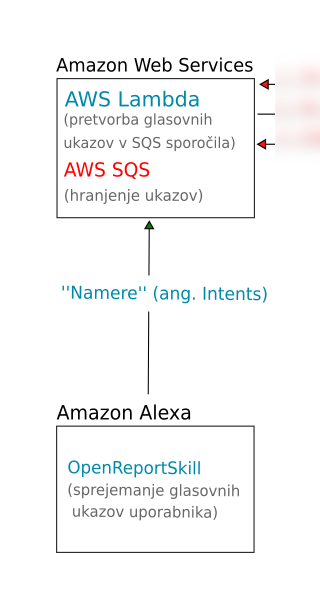
\includegraphics[width=6cm]{plan_alexa_sqs}
\end{center}
\caption{Načrt komunikacije Alexe, AWS Lambda in AWS SQS.}
\label{plan_alexa_sqs}
\end{figure}

Ko uporabnik Alexi izgovori \enquote{Take note \texttt{\{besedilo\}}} ali \enquote{Note \texttt{\{besedilo\}}}, se zažene namera \texttt{TakeNoteIntent} (slika \ref{TakeNoteIntent}).
Polje \texttt{\{besedilo\}} je spremenljivka, v katero veščina hrani razpoznano besedilno vsebino koraka.
Prikaz uporabe: uporabnik izreče \enquote{\textit{note unscrew the backplate}}, torej vrednost spremenljivke \texttt{\{besedilo\}} postane \enquote{unscrew the backplate}.



\begin{figure}[H]
\begin{center}
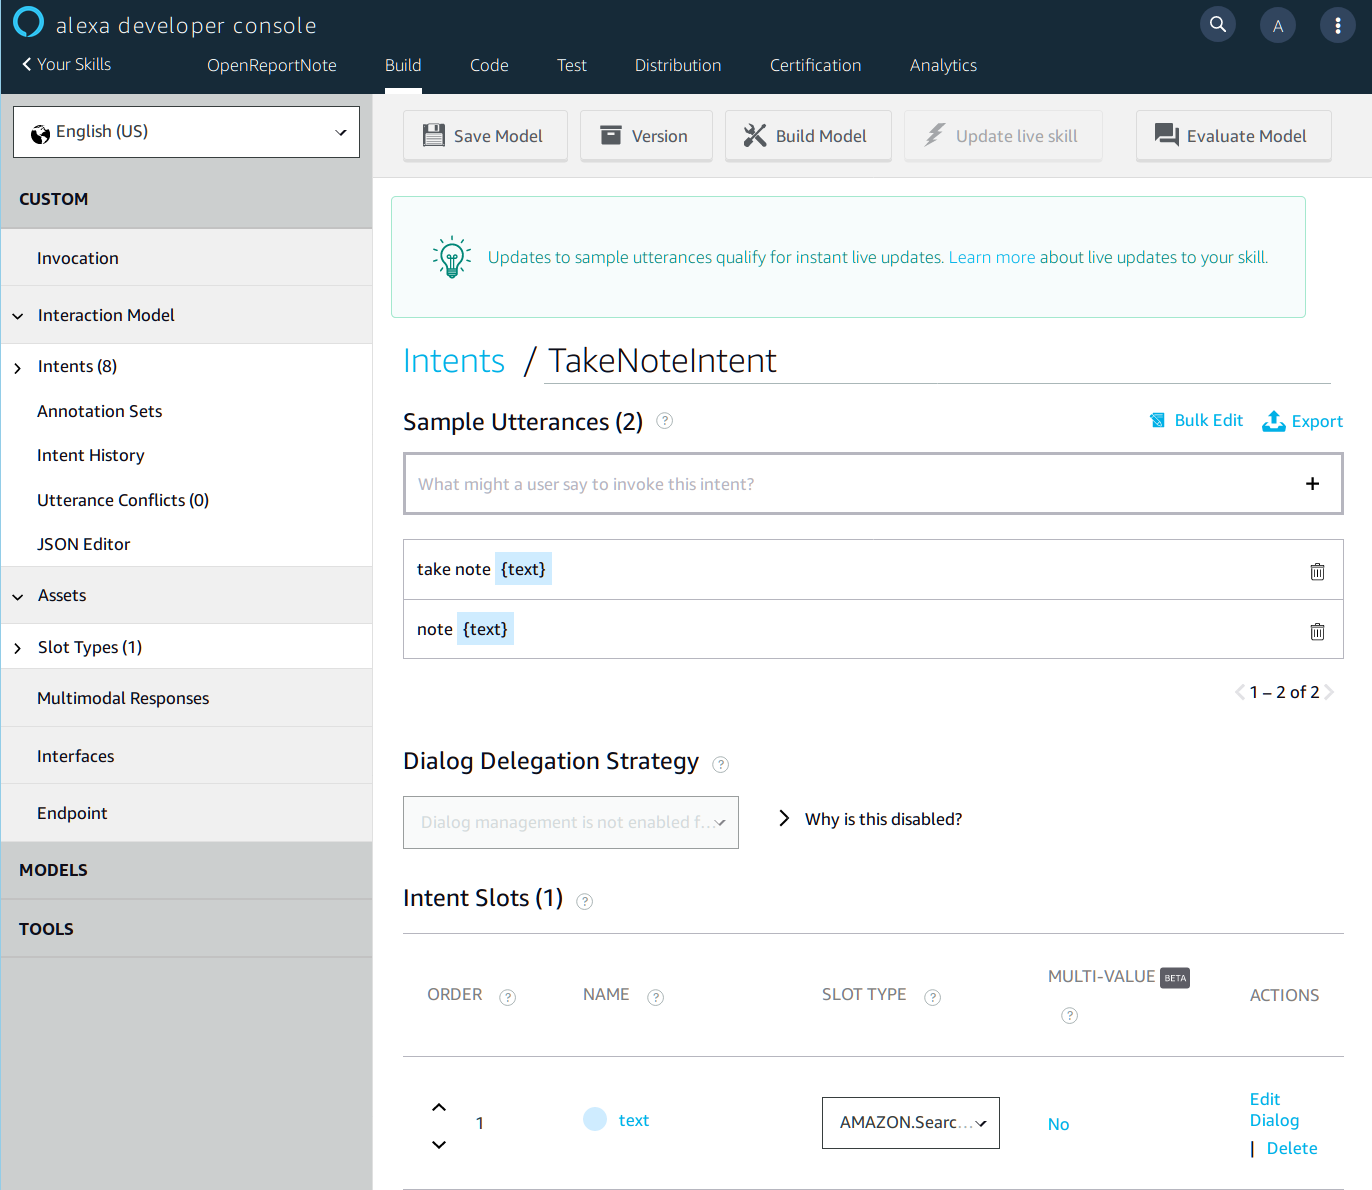
\includegraphics[width=13cm]{intent_literal}
\end{center}
\caption{Fraza TakeNoteIntent v Alexa Developer nadzorni plošči.}
\label{TakeNoteIntent}
\end{figure}

Namera \texttt{TakeNoteIntent} ustvari novo SQS sporočilo, vanj vstavi vrednost spremenljivke \texttt{\{besedilo\}} in ga pošlje na SQS vrsto (implementacija na sliki \ref{skill_code}).
To SQS sporočilo prebere strežnik in ga kot korak vstavi v odprt projekt.
Veščina vrne uporabniku odgovor \enquote{Noted!} in se preneha izvajati.


% j\texttt{OpenTextNoteFormIntent} se zažene, ko uporabnik izreče ukaz za odpiranje obrazca za vstavljanje besedilnega koraka.
% Frazi te namere se glasita \enquote{Create a text note} in \enquote{Add a text note} (slika \ref{OpenTextNoteFormIntent}).

Ko uporabnik Alexi izgovori \enquote{Create a text note} ali \enquote{Add a text note}, se zažene namera \texttt{OpenTextNoteFormIntent}, ki ustvari novo SQS sporočilo, vanj vstavi besedilo \enquote{\texttt{addnote}} in ga pošlje v SQS vrsto.
To SQS sporočilo prebere strežnik in mobilni aplikaciji sporoči, naj odpre obrazec za dodajanje novega besedilnega koraka.
Veščina zatem vrne uporabniku odgovor \enquote{Opening the form!} in se preneha izvajati.

\begin{figure}[H]
\begin{center}
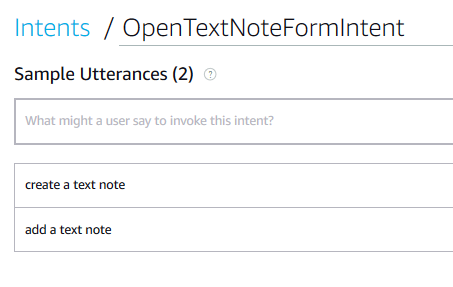
\includegraphics[width=8cm]{intent_text}
\end{center}
\caption{Fraza OpenTextNoteFormIntent v Alexa Developer nadzorni plošči.}
\label{OpenTextNoteFormIntent}
\end{figure}

% DELJENJE
Ko uporabnik Alexi izgovori \enquote{Take a picture}, se zažene namera \texttt{Open-\\ImageNoteFormIntent} (slika \ref{OpenImageNoteFormIntent}), ki se uporablja za prostoročno dodajanje fotografije v delavniški dnevnik.

\texttt{OpenImageNoteFormIntent} ustvari novo SQS sporočilo, vanj vstavi besedilo \enquote{\texttt{addimage}} in ga pošlje v SQS vrsto.
To SQS sporočilo prebere strežnik in mobilni aplikaciji sporoči, naj odpre kamero.
Veščina zatem vrne uporabniku odgovor \enquote{Launching camera!} in se preneha izvajati.

\begin{figure}[H]
\begin{center}
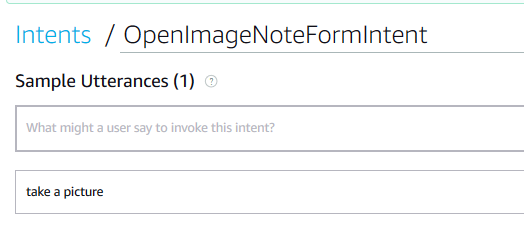
\includegraphics[width=8cm]{intent_image}
\end{center}
\caption{Fraza OpenImageNoteFormIntent v Alexa Developer nadzorni plošči.}
\label{OpenImageNoteFormIntent}
\end{figure}

\begin{figure}[H]
\begin{center}
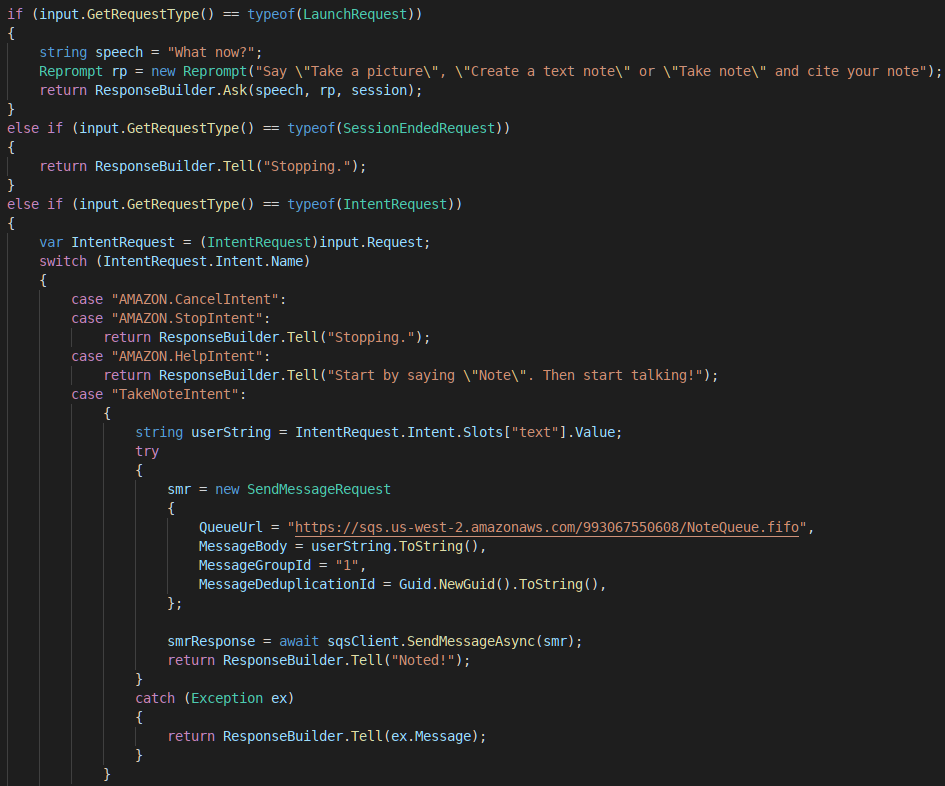
\includegraphics[width=13.5cm]{skill_code}
\end{center}
\caption{Odsek ozadne kode Alexine veščine s prikazom ustvarjanja SQS sporočila.}
\label{skill_code}
\end{figure}

\subsubsection{Prenašanje sporočil med strežnikom in SQS}

Komunikacija strežnika z SQS je prikazana z rdečo barvo na spodnji sliki (slika \ref{plan_sqs_server}).

\begin{figure}[H]
\begin{center}
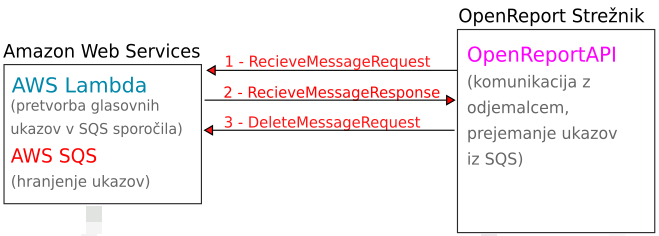
\includegraphics[width=13cm]{plan_sqs_server}
\end{center}
\caption{Komunikacija strežnika z SQS.}
\label{plan_sqs_server}
\end{figure}

Na strežniku OpenReport teče storitev za komunikacijo z glasovnim pomočnikom.
Ta storitev vsakih pet sekund na SQS pošlje zahtevek \texttt{RecieveMessageRequest}.

\begin{Verbatim}[commandchars=+\[\]]
RecieveMessageRequest {
    AttributeName 
    MaxNumberOfMessages 
    QueueUrl 
    WaitTimeSeconds
    ... 
} 
\end{Verbatim}

AWS SQS kot odgovor vrne objekt tipa \texttt{RecieveMessageResponse}.

\begin{Verbatim}[commandchars=+\[\]]
RecieveMessageResponse {
    IEnumerable<Message> Messages;
    ...
}
\end{Verbatim}

V tem odgovoru se nahaja seznam sporočil, ki čakajo na sprejem iz SQS vrste.
V kolikor je v odgovoru vsaj eno sporočilo, pregledamo telo vseh sporočil. 

Ko strežnik sporočila sprejme, jih mora izbrisati iz SQS vrste.
Če jih sproti ne izbriše, iz FIFO vrste ne more brati najnovejših sporočil, ampak le 5 najstarejših.

Sporočila izbriše iz SQS vrste z zahtevkom \texttt{DeleteMessageRequest}.
Ta zahtevek hrani referenco na sporočilo, ki ga želimo izbrisati iz SQS vrste.
AWS SQS storitev v odgovor vrne \texttt{DeleteMessageResponse}, a v tej diplomski nalogi tega odgovora ne uporabimo več.

Zahtevki, ki jih strežnik prejme od glasovnega pomočnika, se odražajo na zadnjem projektu, ki ga uporabnik z glasovnim pomočnikom odpre.
\begin{itemize}
	\item Zahtevek \enquote{\texttt{addnote}} nastavi zastavico \enquote{\texttt{NoteRequest}} na \texttt{true},
	\item zahtevek \enquote{\texttt{addimage}} nastavi zastavico \enquote{\texttt{ImageRequest}} na \texttt{true},
% DELJENJE
	\item zahtevek \enquote{\texttt{\{narekovano besedilo\}}} nastavi zastavico \enquote{\texttt{AlexaNoteRe-\\quest}} na \texttt{true} in prejeto besedilo doda projektu kot korak.
\end{itemize}

\begin{Verbatim}[commandchars=+\[\]]
Project { 
    int Id; 
    string Title; 
    string Description; 
    string Dangers; 
    string FolderLocation; 
    IEnumerable<Note> Notes; 
    +underline[bool NoteRequest;] 
    +underline[bool ImageRequest;] 
    +underline[bool AlexaNoteRequest;] 
}
\end{Verbatim}


Če je vsebina prejetega sporočila enaka \enquote{\texttt{addnote}}, storitev preveri, kateri uporabnik ima trenutno nase vezanega glasovnega pomočnika.
Nato v projektu, ki ga je nazadnje odprl, nastavi vrednost zastavice \texttt{NoteRequest} na \texttt{true}.


Če je vsebina sporočila enaka \enquote{\texttt{addimage}}, storitev preveri, kateri uporabnik ima trenutno nase vezanega glasovnega pomočnika.
V projektu, ki ga je uporabnik nazadnje odprl, nastavi vrednost zastavice \texttt{ImageRequest} na \texttt{true}.

Če vsebina prejetega sporočila ni enaka \enquote{\texttt{addimage}} ali \enquote{\texttt{addnote}}, je prejeto sporočilo dobesedno narekovan korak.
Storitev preveri, kateri uporabnik ima nase vezanega glasovnega pomočnika.
V projektu, ki ga je ta uporabnik nazadnje odprl, nastavi vrednost zastavice \texttt{AlexaNoteRequest} na \texttt{true}.
V ta projekt, se vstavi korak, ki ima naslov \enquote{Voice note}, vsebina pa je telo prejetega sporočila.

\subsubsection{Utemeljitev uporabe SQS}

Prenos sporočil med Amazon Alexo in strežnikom smo realizirali z uporabo storitve AWS SQS.
Pri uporabi SQS je prenos podatkov resda manj učinkovit kot pri direktni povezavi preko spletne vtičnice (\textit{ang. Web Socket}).

Glavni faktor, zaradi katerega smo se odločili za uporabo AWS SQS, je, da z dodatno plastjo za hranjenje sporočil dosežemo enostavno zamenjljivost glasovnega pomočnika.

Pri morebitni menjavi glasovnega pomočnika strežniškega programa ne bi spreminjali.
Potrebno bi bilo le implementirati program za novega glasovnega pomočnika, da na AWS SQS odlaga sporočila v strežniku razumljivem formatu (\enquote{addnote}, \enquote{addimage}).


\subsection{Ovire pri izdelavi Alexa veščine}

Pri implementaciji veščine smo naleteli na veliko težav.

Prva je bila jezikovne narave, saj Alexa ne podpira prepoznavanja slovenskega jezika, zato smo se odločili za uporabo angleškega jezika.

Naslednja težava je bila definicija pozivne fraze.
Fraze, kot so \enquote{take a note} ali \enquote{take a picture} so že rezervirane v sklopu Alexinih privzetih funkcionalnosti, kar pomeni, da jih za našo veščino ne moremo uporabiti.

Izogibati smo se morali tudi frazam, ki so bile rezerviranim frazam podobne (npr. \enquote{open report note} itd.).
Tudi take fraze so se velikokrat razpoznale kot rezervirane fraze.

Težavo je predstavljala izbira poziva, ki je bil hkrati kratek, intuitiven in se ni napačno interpretiral v poziv privzetih funkcionalnosti.
Poziv \enquote{make a report note} je bil najboljši kompromis, ki smo ga našli.

Težavo je predstavljalo tudi razpoznavanje dolgih stavkov, še posebej, če se ti niso ujemali z definiranimi frazami namer.
To je zelo omejilo možnost narekovanja besedila korakov s pomočjo Amazon Alexe.

Naslednjo težavo je predstavljal čas, ki ga je Alexa porabila za interpretacijo definiranih glasovnih ukazov.
Za procesiranje enega glasovnega ukaza je porabila od 3 do 6 sekund.








% \subsection{Zahtevanje in sprostitev glasovnega pomočnika}




\section{Dodelave mobilne aplikacije}

Po implementaciji Alexa veščine smo v mobilni aplikaciji implementirali storitev za upravljanje z glasovnim pomočnikom.
Ta storitev uporabniku omogoča, da lahko zahteva Alexo za delo s svojimi projekti in jo po uporabi sprosti.


\subsection{Zahtevanje in sprostitev glasovnega pomočnika}

OpenReport strežnik podpira delo z enim glasovnim pomočnikom.
Pomočnika lahko uporabnik {zahteva} za lastno uporabo in ga po uporabi {sprosti}.

Ko se zahtevek za uporabo pomočnika potrdi, ga lahko uporabnik uporablja pri sestavljanju delavniškega dnevnika.
Uporabnik lahko glasovnega pomočnika sprosti, kar omogoči drugim uporabnikom, da ga lahko zahtevajo za svoje delo.

Ali ima določen uporabnik nase vezanega pomočnika, vidimo po vrednosti zastavice \texttt{UsesVoiceAssistant} v njegovem objektu razreda \texttt{User}.

Ko uporabnik odpre katerega od svojih projektov, se enolični identifikator tega projekta nastavi v polje \texttt{LastOpenedProjectId} v njegovem objektu razreda \texttt{User}.
Zahtevki, ki jih strežniku pošlje Alexa preko SQS vrste, se navezujejo na projekt s tem identifikatorjem.

\begin{Verbatim}[commandchars=+\[\]]
User : IdentityUser {
    string Id; 
    string Email;
    string Password; 
    IEnumerable<Project> Projects;
    ... 
    +underline[int LastUsedProjectId;]
    +underline[bool UsesVoiceAssistant;]
}
\end{Verbatim}

Uporabnik je pomočnika uspešno zahteval zase, če je \texttt{UsesVoiceAssistant} nastavljen na \texttt{True}.
V mobilni aplikaciji zahtevanje in sprostitev pomočnika nadziramo na {Dashboard} strani, s pritiskom na ikono mikrofona (slika \ref{app_alexa_yesno}).

V aplikaciji za zahtevanje in sprostitev pomočnika skrbi razred \texttt{VoiceAssi-\\stantService.cs}.
Primerek tega razreda se ustvari ob začetku izvajanja aplikacije, nato pa počaka, da avtentikacijska storitev mobilne aplikacije uspešno opravi prijavo uporabnika.

Če ima uporabnik vrednost polja \texttt{UsesVoiceAssistant} nastavljeno na \texttt{true}, ima glasovnega pomočnika vezanega nase in ga lahko uporablja.

Če ima uporabnik vrednost polja \texttt{UsesVoiceAssistant} nastavljeno na \texttt{false}, mora uporabo glasovnega pomočnika zahtevati.
To uporabnik doseže tako, da pritisne na gumb z ikono prečrtanega mikrofona na Dashboard strani (na sliki \ref{app_alexa_yesno} desno).
Ozadna koda aplikacije pošlje avtoriziran PUT zahtevek na URL \enquote{\texttt{/users/requestva}}.

% DELJENJE 
Če nihče od drugih prijavljenih uporabnikov nima polja \texttt{UsesVoiceAssis-\\tant} nastavljenega na \texttt{true}, se njegova zahteva odobri.
V njegovem objektu razreda \texttt{User} se nastavi vrednost \texttt{UsesVoiceAssistant} na \texttt{true}.

Če ima kateri od uporabnikov to polje nastavljeno na \texttt{true}, zahteva ne bo odobrena.
V tem primeru mora uporabnik, ki zahteva pomočnika počakati, da uporabnik, ki pomočnika uporablja, pomočnika sprosti.
Ko si pomočnika ne lasti nihče drug, ga lahko uporabnik zahteva zase.

Uporabnik pomočnika sprosti, ko na strani Dashboard v aplikaciji pritisne gumb z ikono mikrofona.
Ozadna koda aplikacije pošlje PUT zahtevek na URL \enquote{\texttt{/users/releaseva}}.
Na strežniku se nato vrednost polja \texttt{UsesVoiceAssistant} za pošiljatelja zahteve nastavi na \texttt{false}.


\begin{figure}[H]
\begin{center}
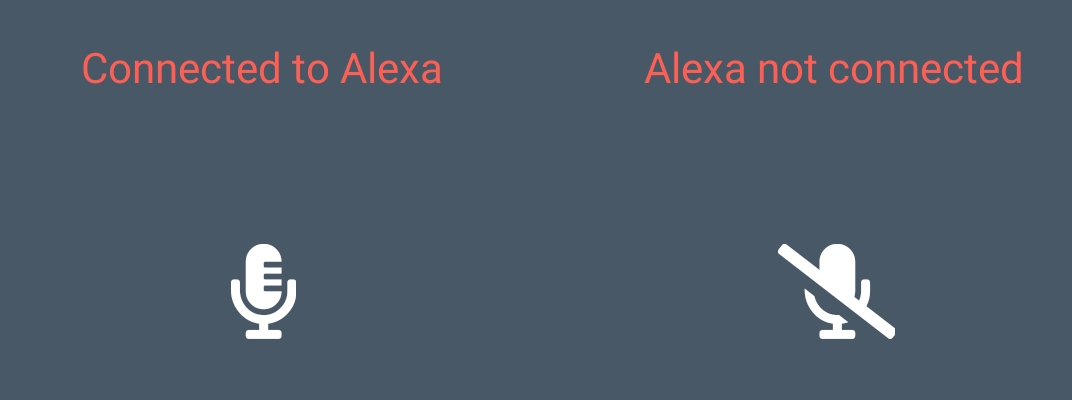
\includegraphics[width=7cm]{app_alexa_yesno}
\end{center}
	\caption{Gumb v obeh stanjih.}
\label{app_alexa_yesno}
\end{figure}




\chapter{Ovrednotenje funkcionalnosti}

Sistem OpenReport smo po končani implementaciji testirali. 
Mobilna aplikacija in strežnik sta izpolnila pričakovanja.

Z mobilno aplikacijo se je bilo možno povezati na strežnik.
Registracija in prijava v sistem preko mobilne aplikacije nista povzročala težav.
Brez težav je delovalo tudi zahtevanje in sprostitev glasovnega pomočnika Amazon Alexe na strani Dashboard.

Delavniške dnevnike je bilo brez težav možno dodajati, odpirati in brisati.

Dodajanje besedilnih korakov v delavniški dnevnik smo ocenili kot smiselno za manjše opombe.
Možnost dodajanja slikovnih korakov v delavniški dnevnik se je izkazala za dobro pri pomembnejših opornih točkah.

Naslove, trajanje in besedilo korakov delavniških dnevnikov smo naknadno spreminjali brez težav.
Urejanje vrstnega reda korakov je delovalo brez težav.
Tudi brisanje korakov delavniškega dnevnika ni povzročalo težav.

Možnost izvoza delavniškega dnevnika v druge formate je delovala brez nevšečnosti.
Ta funkcija lahko olajša prenos podatkov v druge računalniške programe.

\bigbreak

Alexino veščino smo testirali tako, da smo vsako frazo namere izgovorili 20-krat in beležili, kolikokrat se je razpoznala pravilno.
Pri dobesednem narekovanju koraka smo testiranje opravili dvakrat.
Prvič smo testirali s stavkom \enquote{\textit{this is a voice note}}, drugič pa s stavkom \enquote{\textit{backplate removal takes about three minutes}}.
\begin{itemize}
	\item Alexa je ukaz \enquote{\textit{take a picture}} pravilno razpoznala v 18 od 20 testnih izgovorjav.
	\item Ukaz \enquote{\textit{create a text note}} je pravilno razpoznala v 17 od 20 testnih izgovorjav.
	\item Ukaz \enquote{\textit{note this is a voice note}} je pravilno razpoznala v 3 od 20 testnih izgovorjav.
	\item Ukaza \enquote{\textit{note backplate removal takes about three minutes}} ni pravilno razpoznala v nobeni od 20 testnih izgovorjav.
\end{itemize}
Narekovanje besedila glasovnemu pomočniku ni izpolnilo pričakovanj.
Rezultati testiranja razpoznavanja glasovnih ukazov so pokazali, da v našem primeru Alexa veliko bolje razpoznava fraze, ki se z definirano frazo namere v celoti ujemajo kot tiste, ki nimajo velike stopnje ujemanja.

Dodajanje slikovnih in besedilnih korakov s pomočjo glasovnega ukaza se je izkazalo za delno uspešno.
Alexa je v teh primerih ukaze razpoznavala z zadovoljivo natančnostjo.
Za uporabno se je izkazalo predvsem, ko mobilnega telefona med delom nismo imeli na dosegu roke.
Vseeno pa je predstavljal težavo čas, ki bil je potreben, za izgovorjavo poziva, fraz namer in čakanje na obdelavo zahtev.
To je trajalo v povprečju 18 sekund, kar smo ocenili kot prepočasno za učinkovito uporabo.

Odklepanje mobilnega telefona, ki ga smo ga imeli v dosegu roke ter odpiranje obrazca za dodajanje korakov je trajalo v povprečju 4 sekunde.
Odklepanje mobilnega telefona, ki je bil oddaljen tri metre ter odpiranje obrazca za dodajanje korakov je trajalo v povprečju 8 sekund.

Težavo je predstavljalo tudi, če uporabnik ni znal angleškega jezika.

Naposled smo ugotavili, da je za zasnovo sistema, ki vključuje Amazon Alexo, treba skrbno upoštevati Alexine omejitve.
V našem primeru smo dobro prepoznavanje ukazov dosegli pri ukazih brez spremenljivih členov.
Sklepamo lahko, da bi se sprejemljivo obnesla v sistemih, kjer so glasovni ukazi statično definirani.

Kljub nekaterim pomanjkljivostim pa smo razvili funkcionalen sistem, ki lahko služi kot dobra osnova za nadaljnji razvoj.
Sistem smo lahko namreč tudi brez glasovnega pomočnika uporabljali za učinkovito sestavljanje delavniških dnevnikov.




\chapter{Zaključek}

Sistem, razvit v sklopu diplomske naloge, zajema funkcionalosti, ki uporabniku omogočajo sestavljanje delavniških dnevnikov.
Sestavljajo ga strežnik, mobilna aplikacija in glasovni pomočnik Amazon Alexa.
Uporabnik lahko v delavniške dnevnike dodaja preproste besedilne korake.
Z uporabo mobilne aplikacije lahko zajame fotografije in jih v delavniški dnevnik vstavi kot slikovno gradivo.

Ta sistem je služil kot primer sistema, ki ga želimo izboljšati z uporabo glasovnega pomočnika.
Naš namen je bil poenostaviti delo s sistemom, z uvedbo glasovnega pomočnika Amazon Alexe.
Implementirali smo odpiranje kamere in obrazca za dodajanje korakov z glasovnim pomočnikom.
Kljub uspešni implementaciji je bil čas, potreben za izgovorjavo in obdelavo glasovnih ukazov, predolg, da bi poskus izboljšave bil popolnoma uspešen.
Za neuspešno se je izkazalo glasovno narekovanje vsebine koraka delavniškega dnevnika.
Z Amazon Alexo ni bilo mogoče razpoznati daljših, spremenljivih stavkov.

V možne izboljšave sistema smo na prvo mesto uvrstili preizkus drugih glasovnih pomočnikov, npr. Google Assistant \cite{googleass}.
%Hitrejše upravljanje z aplikacijo bi lahko dosegli z pomočnikom, ki bi lahko razpoznal ukaze z eno samo frazo in ne kombinacijo dveh, kot Amazon Alexa.
Druga smiselna izboljšava je izvoz delavniških dnevnikov v več različnih standardnih formatov, kot so npr. XSL ali ODS.

Mobilna aplikacija in strežniški program sta zadovoljila pričakovanja in lahko že v trenutnem stanju služita kot referenca za primerjavo učinkovitosti Amazon Alexe in drugih glasovnih pomočnikov.

Kljub nekaterim težavam z uporabo glasovnega pomočnika je očitno, da je tehnologija glasovnih pomočnikov zelo primeren način za nadzor sistemov na daljavo.
Poleg tega ponuja veliko možnosti za slepe, slabovidne in gibalno omejene posameznike, ki imajo težave pri interakciji z računalnikom.




\newpage %dodaj po potrebi, da bo številka strani za Literaturo v Kazalu pravilna!
\ \\
\clearpage
\addcontentsline{toc}{chapter}{Literatura}

\printbibliography

\end{document}
